%% This is an example first chapter.  You should put chapter/appendix that you
%% write into a separate file, and add a line \include{yourfilename} to
%% main.tex, where `yourfilename.tex' is the name of the chapter/appendix file.
%% You can process specific files by typing their names in at the 
%% \files=
%% prompt when you run the file main.tex through LaTeX.


\chapter{Microzooplankton community structure investigated with imaging flow cytometry and automated live-cell staining}

Emily F. Brownlee$^{1,2}$, Robert J. Olson$^{2}$, Heidi M. Sosik$^{2}$\\                                                         
$^{1}$MIT-WHOI Joint Program in Oceanography/Applied Ocean Science and Engineering, Cambridge, MA 02142, USA\\
$^{2}$Biology Department, Woods Hole Oceanographic Institution, Woods Hole, MA 02543, USA\\

Available online: Brownlee, E.F., R.J. Olson, H.M. Sosik. 2016. Microzooplankton community structure
investigated with imaging flow cytometry and automated live-cell staining. Marine Ecology
Progress Series. 550:65-81. doi:10.3354/meps11687

\section{Abstract}

Protozoa play important roles in grazing and nutrient recycling, but quantifying these roles has been hindered by difficulties in collecting, culturing, and observing these often-delicate cells. During long-term deployments at the Martha's Vineyard Coastal Observatory (Massachusetts,
USA), Imaging FlowCytobot (IFCB) has been shown to be useful for studying live cells in situ without the need to culture or preserve. IFCB records images of cells with chlorophyll fluorescence above a trigger threshold, so to date taxonomically resolved analysis of protozoa has presumably
been limited to mixotrophs and herbivores which have eaten recently. To overcome this limitation, we have coupled a broad-application \lq{live cell}\rq fluorescent stain with a modified IFCB so that protozoa which do not contain chlorophyll (such as consumers of unpigmented bacteria
and other heterotrophs) can also be recorded. Staining IFCB (IFCB-S) revealed higher abundances of grazers than the original IFCB, as well as some cell types not previously detected. Feeding habits of certain morphotypes could be inferred from their fluorescence properties: grazers
with stain fluorescence but without chlorophyll cannot be mixotrophs, but could be either starving or feeding on heterotrophs. Comparisons between cell counts for IFCB-S and manual light microscopy of Lugol's stained samples showed consistently similar or higher counts from IFCB-S.
We show how automated classification through the extraction of image features and application of a machine-learning algorithm can be used to evaluate the large high-resolution data sets collected by IFCBs; the results reveal varying seasonal patterns in abundance among groups of protists.

\section{Introduction}

Heterotrophic protists are significant in marine ecosystems; they mediate top-down control of primary producers, as well as playing central roles in the microbial loop and food web (Heinbokel \& Beers 1979, Lessard \& Swift 1985, Verity 1985, 1991, Jacobson \& Anderson 1986, Stoecker \& Capuzzo 1990, Bj�rnsen \& Kuparinen 1991, Hansen 1991). These microzooplankton have not been studied as extensively as other plankton, however, because it is typically time-consuming and difficult to enumerate and identify them. Many are fragile and net collection can be harmful to their structure. Furthermore, their soft bodies make preservation difficult due to shrinkage and distortion or disintegration (Stoecker et al. 1994). Certain types of preservation can also lead to lysis and egestion of food vacuole contents (Sieracki et al. 1987). Protozoa are challenging to culture due to their complex nutritional needs. Because of these difficulties, long-term, high-resolution data sets are rare. This limits our ability to characterize how their abundance and community structure respond to natural variations such as seasonality and longer-term trends associated with environmental and climate change. 

New technology that combines microscopy and flow cytometry promises to overcome some of these observational challenges by enabling high temporal resolution sampling for long periods of time. Imaging FlowCytobot (IFCB), which uses laser-induced fluorescence to trigger capture of images of individual plankton, is one such system (Olson \& Sosik 2007). While IFCB was originally designed to characterize phytoplankton, it can also be used to study herbivorous and mixotrophic protozoa in situ without the need to culture or preserve. Herbivorous protozoa ingest phytoplankton that can continue to fluoresce inside food vacuoles. Kleptoplastidic and mixotrophic protozoa are also fluorescent because they retain functional chloroplasts to supplement their nutrition.

Complete protozoan assemblages are traditionally counted and identified by epifluorescence microscopy of samples stained with protein or nucleic acidstains. These traditional methods quantify not only herbivorous microzooplankton, but also those grazing on non-chlorophyll-containing cells. To observe the complete heterotroph community, imaging methods must employ triggering on a property common to all grazers. Such triggering can be provided by \lq{live cell}\rq \hspace{0.2cm}fluorescent stains such as LysoTracker$^{\circledR}$Green (LTG) (Molecular Probes) or fluorescein diacetate (FDA) (Sigma-Aldrich). FDA permeates the cell to fluoresce in the presence of enzymatic activity. LTG accumulates within acidic food vacuoles so actively grazing protists can be distinguished. These stains accumulate within living cells to provide high signal-to-noise. Phototrophs can take up stain, but in cytometric analyses they can be differentiated from heterotrophs by their relatively high levels of red auto fluorescence from chlorophyll. Heterotrophs with chloroplasts in their food vacuoles may also express red autofluorescence, but typically at lower levels than autotrophs of similar size. Since IFCB is normally limited to detecting herbivorous or mixotrophic protozoa, the use of a stain to view a more complete community represents a powerful advance for this observational technique. 

Here we use ciliate cultures and environmental samples to demonstrate the capabilities and performance of an IFCB modified for automated staining (IFCB-S). We also demonstrate the use of automated classification to analyze the resulting large data sets. We find automated imaging with the addition of staining allows for detection of a greater number and diversity of grazers and may also provide insight into feeding habits.

\section{Materials and Methods}

\subsection{Instrument design}\label{ch2:opts}

We modified a standard IFCB to carry out automated staining and incorporated optical components that enable it to detect either orange (as from phycoerythrin, PE) or green (stain) fluorescence, in addition to chlorophyll fluorescence. The optical and fluidic design for IFCB has been described in detail in Olson \& Sosik (2007). A sample (typically 5 ml) is drawn into the instrument by a programmable syringe pump. The sample water is injected into the center of a particle-free sheath flow in the cone above a rectangular quartz flow cell. In the standard IFCB, seawater is drawn into a sample syringe and then injected directly into the cone through a needle; after the flow cell, particles are removed by passage through cartridge filters to regenerate sheath fluid. For IFCB-S, we added new fluidics control features utilizing IFCB's distribution valve and new solenoid valves (100T2NC24-62-4E, Bio-Chem Valve) to allow for automated addition of stain, as well as for discarding sheath fluid during stained sample analysis (to prevent accumulation of
stain in the system). Staining is carried out in a mixing chamber (a 50 ml Falcon tube fitted with plumbing) connected to an extra port on the valve. First, a microinjector (120SP2420-4EE, Bio-Chem Valve) adds 20 $\upmu$l of concentrated stain to the empty chamber. Then the seawater sample is pushed through the distribution valve into the mixing chamber, where it mixes with the stain and incubates (typically for 30 s) before being pulled back into the sample syringe and sent through the flow cell for analysis (Fig. 1). 

Standard IFCB excites chlorophyll fluorescence with a 635 nm diode laser (details in Olson \& Sosik 2007). As a particle passes through the focused laser, laser light is scattered and chlorophyll-containing cells emit red fluorescence (680 nm). One (or more) of these signals, usually chlorophyll fluorescence, is used to trigger a 1 $\upmu$s pulse from a xenon flash lamp. The green component of the lamplight is isolated by a bandpass filter and used for the camera exposure. Dichroic mirrors separate the wavelengths used to detect chlorophyll fluorescence and side scattering
(680 nm and 635 nm, respectively). In the modified optics for IFCB-S (Fig. 2), the 635 nm laser is replaced by a 508 nm diode laser (Power Technology, model PM20(510-50)G4, 20 mW) that can excite fluorescence from the stain (530 nm), as well as from chlorophyll (680 nm) and phycoerythrin (575 nm). A 488 nm laser can also be used for this set-up, though it utilizes more power than the 508 nm laser. In this case, a 570 nm shortpass filter is inserted before the photomultiplier
tube that detects PE because 488 nm excitation causes Raman scattering from water at ~590 nm. We incorporated an automated optical filter slider making it possible to detect either orange (PE) fluorescence for unstained samples or green (stain) fluorescence for stained samples. To detect stain fluorescence, IFCB-S uses a \lq{double dichroic}\rq\hspace{0.1cm}(Omega Optical, 595 DMSP), which transmits light between 560 and 595 nm to the camera and reflects light below and above this band to the photomultiplier tubes. To detect PE fluorescence (when samples are not stained), IFCB-S uses a 555 DMSP, which transmits 530 to 570 nm and reflects longer wavelengths.


\subsection{Staining validation}

We used a cultured marine bacterivorous scuticociliate (\textit{Uronema marinum}, isolated from Buzzards Bay, MA, in 1986; D. Caron pers. comm.) to evaluate initial IFCB-S performance. Cultures were maintained at 15$^{\circ}$C on a 14:10 h light:dark cycle and transferred weekly into 40 ml sterile filtered seawater with 1 drop yeast extract and 2 rice grains. As a control, scuticociliate cells were imaged with IFCB-S triggering on scattering to ensure detection of all cells. To evaluate stain detection, cells were then analyzed with IFCB-S triggering only on stain fluorescence with and without stain added.

\subsection{IFCB-S stain protocol}

To select an appropriate stain concentration, various stock stain concentrations (0, 0.01, 0.05, 0.1, 1, 2 mg FDA ml$^{-1}$ acetone) were tested on a scuticociliate culture analyzed with IFCB-S triggering on stain fluorescence. As a control, an unstained sample (stock stain concentration of 0 mg FDA ml$^{-1}$ acetone) was triggered on scattering. For each stock concentration, we added 8 $\upmu$l of stain to a 2 ml sample prior to analysis on IFCB-S. This resulted in final stain concentrations of 0, 0.04, 0.2, 0.4, 4, and 8 $\upmu$g FDA ml$^{-1}$. Once a final stain concentration was chosen, an additional 5 ml sample of scuticociliate culture was stained and analyzed with triggering on stain fluorescence to determine if stain fluorescence values are stable over the time course of analysis (20 min).

\subsection{Stain comparison}

To compare detection efficiency between LTG and FDA, scuticociliate cultures were sampled daily during batch growth, and cell counts were determined with a FACSCalibur$^{TM}$ flow cytometer. Each day the scuticociliate culture was analyzed 3 ways; unstained and triggering on side scattering, stained with LTG and triggered on stain fluorescence, and stained with FDA and triggered on stain fluorescence. We withdrew 2 ml subsamples of the culture and added either 8 $\upmu$l of FDA solution (1 mg ml$^{-1}$ stock solution in acetone for a final concentration of 4 $\upmu$g ml$^{-1}$) or 1.25 $\upmu$l of LTG solution (1 mM stock diluted to 12 $\upmu$M working stock for a final stain concentration of 75 nM). For each run through the FACSCalibur, 120 $\upmu$l was analyzed over 2 min.

\subsection{Comparison with conventional microscopy }

Seawater samples were collected from Woods Hole Harbor (Massachusetts, USA). Samples were kept at in situ temperature for approximately 6 h while aliquots were taken for analysis on IFCB-S in staining and non-staining modes (50 ml were analyzed in total by pooling results from ten 5 ml subsamples). For manual microscopic counts, 200 ml of the sample was fixed with 10 ml acid Lugol's solution (final concentration 5\%, modified from Throndsen 1978). Acid Lugol's-fixed samples (50 ml) were settled for 24 h in Uterm�hl chambers and cells were subsequently enumerated under a Zeiss Axiovert S100 inverted microscope at 40� magnification.

Microzooplankton counts from manual light microscopy were compared to those from IFCB-S in staining mode (triggering on chlorophyll and stain fluorescence) and IFCB-S in non-staining mode (triggering on chlorophyll and PE fluorescence). For these comparisons, ciliates were grouped into 4 taxonomic categories: tintinnids, \textit{Mesodinium} spp., \textit{Laboea strobila}, and \lq{other ciliate taxa}\rq. The heterotrophic dinoflagellates, \textit{Gyrodinium} spp. and \textit{Protoperidinium} spp. were also considered for comparison. Analyses were performed during all 4 seasons; winter, spring, summer, and fall (with the winter and fall sample lacking manual light microscopy). Poisson distribution statistics were used to calculate 95\% confidence intervals for counts. The E-Test statistic described by Krishnamoorthy \& Thomson (2004) was used to test for significant differences.

\subsection{Comparison of detection between IFCB and IFCB-S}

For field assessment, IFCB-S was used during the National Marine Fisheries Service Ecosystem Monitoring survey (ECOMON, EX-13-05) aboard the NOAA Ship  \lq{Okeanos Explorer}\rq from August 24 to September 5, 2013. The cruise track covered the continental shelf from southern New England waters northward through Georges Bank and the Gulf of Maine to Nova Scotia shelf waters. IFCB-S was used side-by-side with a standard IFCB for continuous sampling of water from the ship's underway system (3 m sample depth). The standard IFCB triggered on chlorophyll fluorescence, while IFCB-S was configured to alternate between staining (triggering on chlorophyll and/or stain fluorescence) and nonstaining (triggering on chlorophyll and/or PE fluorescence) modes.

\subsection{Automated classification of a time series}

Since 2006, standard IFCB has been deployed underwater ($\sim$ 4 m depth) at the offshore tower of the Martha's Vineyard Coastal Observatory (MVCO), located 3 km south of Martha's Vineyard, Massachusetts, USA. At MVCO, IFCB has provided near continuous long-term observations (2006 to present) of phytoplankton ranging from $\sim$ 10 to 400 $\upmu$m in length, as well as herbivorous and mixotrophic ciliates that exhibit chlorophyll fluorescence. Routine analysis of IFCB data includes image processing, feature extraction, and supervised automated classification as described by Sosik \& Olson (2007) except that instead of the original support vector machine, we used a random forest classification algorithm after Breiman (2001). We applied a classifier with 50 categories, including L. strobila, mixed tintinnids, and mixed other ciliates. For each unknown image, results from the classification algorithm (Tree-Bagger function in MATLAB, The Mathworks) provide an affiliation score for each category (scores sum to 1 across all categories). By selecting a score threshold above which classifications are accepted, it is possible to reduce the incidence of false positives, albeit typically at the expense of lower probability of detection for true positives. The efficacy of this approach is demonstrated here by comparing intermittent manual image identification with a high-resolution multi year time series of cell abundance from the automated classifier for the ciliate species  \textit{L. strobila} at MVCO.  \textit{L. strobila} was chosen as a target because it has distinct morphology, it is typically among the top 5 contributors to micrograzer biomass on an annual basis at MVCO, and it exhibits seasonal patterns that we want to characterize with high resolution. Linear regression analyses between manual and automated counts for various score thresholds were performed and values of R$^{2}$, y-intercept, and slopes were used to select a threshold score. An ideal threshold would be one where the R$^{2}$ is maximized, the y-intercept is near zero, and the slope approaches 1. Once a threshold score is selected, abundance estimates are determined by counting targets with scores above that cut-off, and an average correction efficiency is applied by dividing the total by the regression slope for the chosen threshold.

\section{Results}

\subsection{Imaging of protozoa}
The level of taxonomic identification allowed by IFCB images varies, but some distinctive taxa, such as Laboea strobila, can be identified to the species level. At MVCO, the predominant ciliates detected by the standard IFCB come from the Spirotrichea subclasses Oligotrichia and Choreotrichia (Fig. 3). The photosynthetic ciliate \textit{Mesodinium} spp. is also readily detected due to its mixotrophic nature. More rare ciliate taxa include the haptorid \textit{Didinium} spp. and the prostomatid \textit{Tiarina fusus}. 

Heterotrophic dinoflagellates are also detected if they are consuming phytoplankton (Fig. 4). These are predominantly gyrodinoid and gymnoid forms. Occasionally \textit{Protoperidinium} spp. and \textit{Amphidinium} spp. are observed.

The instrument can capture images of cells or chains up to at least 400 $\upmu$m, though sampling is limited to cells <150 $\upmu$m in width.

All images from the MVCO data set can be viewed and accessed through the IFCB Data Dashboard (Sosik \& Futrelle 2012; http://ifcb-data.whoi.edu/mvco). All annotated ciliate and dinoflagellate images (organized by year and taxonomic group) are available from the published WHOI-Plankton data set (Sosik et al. 2015). Heterotrophic dinoflagellates are also detected if they are consuming phytoplankton (Fig. 4). 

\subsection{Performance of IFCB-S}
To evaluate the ability of IFCB-S to stain and detect ciliates lacking chlorophyll fluorescence, we used a bacterivorous scuticociliate culture. On a standard IFCB triggering on chlorophyll fluorescence, these ciliates do not trigger image capture, so initially we used a side-scattering trigger to detect all particles (Fig. 5A). In this case, both detrital particles and ciliates were imaged, with detrital particles dominating but ciliates readily detectable. When a non-stained cell culture was analyzed on IFCB-S configured to trigger on stain fluorescence, no scuticociliates were detected, as expected, since these cells do not exhibit detectable autofluorescence (Fig. 5B). Once cells were stained, they were readily detected with a stain fluorescence trigger (Fig. 5C). Triggering on stain fluorescence rather than scattering increases the time spent imaging ciliates as opposed to detritus (75\% of the fluorescence-triggered images contained ciliates compared to only 41\% of scattering-triggered images).

\subsection{Comparison of stains}
To compare the performance of LTG and FDA, scuticociliate cell counts were determined by conventional flow cytometry triggering on stain fluorescence. Detection efficiency was similar between the 2 stains (Fig. 6), allowing for further considerations to be used in selecting the optimal stain for use in IFCB-S. We selected further application of FDA due to its stability in solution for up to 6 mo at room temperature (pers. obs.), as well as its lower cost. Recommended storage for LTG is -5 to -30$^{\circ}$C, which presents challenges for long-term in situ deployments.

\subsection{Determining stain protocols}
We found the average stain fluorescence levels of scuticociliates measured by IFCB-S increased until leveling off at a final stain concentration of 4 $\upmu$g FDA ml$^{-1}$ (Fig. 7A). The unstained sample displayed low levels of stain fluorescence, representing instrument noise. We chose the final concentration of 4 $\upmu$g FDA ml$^{-1}$ for use in the IFCB-S system to maximize sensitivity without introducing excess stain that could contaminate the instrument?s fluidic system and require extra rinsing to remove.

The time course of cell stain fluorescence during the 20 min analysis of a 5 ml scuticociliate culture sample showed a slight increase of average stain fluorescence over the first 6 min of the sample and a slight decrease over the last 6 min (Fig. 7B). All cells stained, though, were above the detection level and whole cell counts per 30 s bin remained constant until a small increase in the last 2 min of the sample. That increase may partially be due to cells concentrating near the top of the syringe and being analyzed later in the time course. The counts from the first 30 s bin are low due to small amounts of particle-free sheath fluid from previous rinses remaining in the needle. Ultimately, this verifies 30 s is adequate for staining all cells prior to analysis, though highest
staining occurs several minutes later.

\subsection{Comparison of IFCB-S and manual microscopy}
We evaluated performance of IFCB-S on environmental samples by comparison with the conventional mode of counting protozoa: settling and using manual microscopy to count cells in acid Lugol?s stained samples. We also compared IFCB-S counts with staining (chlorophyll and stain fluorescence trigger) and without staining (chlorophyll fluorescence trigger only). We specifically compared abundances for \textit{Mesodinium} spp., \textit{L. strobila}, mixed tintinnids, \textit{Protoperidinium} spp., and mixed gyrodinoid dinoflagellates. During a comparison of wintertime samples, no significant differences were found between ciliate morphotypes detected by IFCB-S with and without staining (Fig. 8A). In stained samples, however, more gyrodinoid dinoflagellates were detected, indicating these organisms are likely consuming heterotrophs and thus often missed by standard IFCB with a chlorophyll trigger (Fig. 8A). During a springtime comparison, IFCB-S detected approximately 25\% more mixed ciliates than microscopic analysis (Fig. 8B). At that time, there were no significant differences in abundances for other micrograzer morphotypes between the methods. There were also no differences in detection between staining and non-staining modes (Fig. 8B), consistent with most protists containing chlorophyll either in their guts or in retained plastids. A summertime sample allowed only for comparison in the ciliate mix and tintinnid groups as other types were not observed (Fig. 8C). For the detected ciliate types, both stained and unstained sample concentrations were significantly higher than manual microscopy. A fall comparison did not show any significant differences between staining and non-staining modes
(Fig. 8D).
 
\subsection {IFCB-S field application}
IFCB-S was configured for automated underway sampling of surface waters during a cruise over the northeast US continental shelf (August 2013). We examined ciliate and gyrodinoid dinoflagellate abundance and compared morphotypes that did and did not ingest algae. Two populations of organisms were observed in the stained samples: one with high chlorophyll fluorescence and one with little to no chlorophyll fluorescence; both showed a range of stain fluorescence that roughly corresponded to cell size. Ciliates and dinoflagellates were present in
both of these groups, so it was possible to detect a greater number of total grazers in stained samples. This was due to taxa present in the low red / high stain fluorescence population (Fig. 9).

Observations of tintinnids during the cruise provided a notable example of the advantages of IFCB-S. We found 2 morphologically different groups of tintinnids in the stained samples: one with high
chlorophyll fluorescence and one with little to no chlorophyll fluorescence; as expected, both groups exhibited stain fluorescence. Only chlorophyll fluorescent tintinnids were detected by the standard IFCB, with maximum concentrations reaching approximately 0.4 cells ml$^{-1}$ (Fig. 10A). This population was captured by IFCB-S in similar concentrations, but the second population with little chlorophyll fluorescence was detected only by this instrument, with resulting higher total tintinnid maximum abundances determined by IFCB-S compared to IFCB ($\sim$ 1.1 cell ml$^{-1}$) (Fig. 10B). The staining of samples consistently allowed for detection of a group of tintinnids that otherwise would not have been observed.

\subsection {Automated classification}
Automated classification is essential for analyzing the large data sets produced by IFCB and IFCB-S. We explored the automated approach for ciliates by comparing manual and automated identification of images for times series data from 2006 to 2015 for \textit{L. strobila}. Regression analysis between manual and automated classification results (Fig. 11) suggested an optimal classifier score threshold of 0.7 (i.e. an image is classified as \textit{L. strobila} only if the score associated with the class is >0.7): the R$^{2}$ value was high, the y-intercept was not significantly different from 0, and the slope was relatively close to 1. This 0.7 threshold produced an acceptable tradeoff between detection efficiency and occurrence of false positives. This tradeoff is reflected in the performance statistics of the classifier, which for the case of the random forest method we used can be determined from the unbiased internal error rates (out-of-bag estimates that do not require a separate test set; Breiman 2001). From this approach, our classifier has a probability of detection = 0.97 and precision = 0.90 for the \textit{L. strobila} class before application of any score threshold. With the selected score threshold of 0.7, the corresponding probability of detection drops to 0.79 (19\% unclassified and 2\% misclassified), while the precision increases to 0.99. These rates are consistent with performance on the full set of manually labeled images, where the intercept
between automated and manual counts is $\sim$0 and the slope is 0.75 (Fig. 11A).

Automated and manual classification of the MVCO images provided similar patterns of variability with both showing distinct seasonal patterns in \textit{L. strobila} abundance (Fig. 12). At finer scales, there can be discrepancies between automated and manual identification. Some of these discrepancies may be caused by patchiness at MVCO interacting with sampling differences: in some cases, manual classification was only completed for a few hours within a given day, while the daily estimate for automated classification reflects sampling over the entire day. If different water masses were moving by the MVCO offshore tower throughout the day, high frequency variability in cell concentration might lead to mis-matches with the resulting daily average values. For event- to seasonal-scales, fully automated abundance estimates provide robust patterns, with blooms of \textit{L. strobila} occurring during April-May in most years, and some evidence for fall blooms that are smaller and more

\section{Discussion}
Protist micrograzers are key players in aquatic ecosystems yet they are difficult to study due to methodological challenges. The standard IFCB is a powerful tool for studying these organisms in situ. Because IFCB can be deployed long-term, it is effective for characterizing protozoan community structure with high temporal resolution. It can image a wide variety of grazers and provide insight into which organisms are present (e.g. Figs. 3 \& 4), as well as their seasonal dynamics (Fig. 12). There are limitations, though, because the reliance on chlorophyll fluorescence for image triggering means standard IFCB is only able to quantify patterns of herbivores and mixotrophs. The addition of broad-application live cell staining is appropriate to take this observational technique forward to view a more complete community.

In typical cytometric analyses, there can be difficulty when discriminating a phototroph with concentrated stain from an herbivorous or mixotrophic protozoan because both can have high levels of chlorophyll fluorescence. Imaging technology allows us to differentiate the two from the images associated with each cell. On the other hand, some grazers may have undetectable levels of chlorophyll fluorescence or none at all (for instance, those grazing on heterotrophs) and the addition of stain is necessary for efficient detection. There are a number of possible fluorescent
stains that can be used to label protists for flow cytometry. We considered several factors in selecting a stain for use with IFCB-S, including whether the stain fluorescence can be differentiated from chlorophyll and can remain stable at ambient temperatures (important for long-term in situ deployments). Most importantly, the wavelength of the laser must be able to induce fluorescence by the stain, but limit overlap of emitted wavelengths with scattered laser light. This criterion led us to focus on LTG and FDA as candidates. While suggested final FDA concentrations vary (Dorsey et al. 1989, Jochem 1999, Onji et al. 2000, Peperzak \& Brussaard 2011, 0.06-500 $\upmu$g FDA ml$^{-1}$), we recommend use of FDA for extended in situ staining application at a final concentration of 4 $\upmu$g FDA ml$^{-1}$. Though 30 s of staining is adequate to stain all cells (so appropriate for most analyses), if maximum stain accumulation is desired, stained samples should be incubated for 2-6 min before analysis and sample analysis time should be limited to 10-15 min. FDA's effectiveness is comparable to that of LTG (Fig. 6), while its ability to remain stable at ambient temperatures (Boyd et al. 2008 and pers. obs.) and its affordability make it preferable. Because LTG stains the acid vacuoles created during digestion (Rose et al. 2004), it might be useful to distinguish those protists that are actively grazing, but our observations showed general staining of all cells including pure autotrophs (likely because chloroplasts can be acidic) and not in relation to levels of grazing. With controlled analysis of a bacterivorous scuticociliate culture, we have shown that automated staining can be used to readily detect and image grazers previously undetectable with IFCB (Fig. 5). While the degree of staining may be variable for different grazers, our results suggest that widespread detection of grazers without chlorophyll fluorescence is possible.

To test the effectiveness of protozoa detection by automated imaging in mixed assemblage natural
samples, we compared results to those from manual light microscopy. For samples collected from Woods Hole Harbor in spring and summer, significantly higher abundances of mixed ciliates were detected with IFCB-S compared to manual microscopy (Fig. 8B,C). This suggests traditional counting methods involving preservation and settling may be so detrimental to the cells that they become undetectable. This is consistent with the conclusions of Stoecker et al. (1994) that no
single method of fixation is ideal for all purposes, so taxon- and fixation-specific correction factors may need to be applied for methods that involve preservation. Because the IFCB is used to image ciliates in situ without fixation steps, loss of delicate cells may be minimized. In no cases did we observe significantly lower concentrations of any organisms with the IFCB or IFCB-S compared to manual microscopy. This is consistent with previous findings for various types of phytoplankton (Olson \& Sosik 2007, Campbell et al. 2010, Brosnahan et al. 2015). The instrument was not been found to be biased towards certain morphotypes over others, as the range of microzooplankton detected with the IFCB-S did not differ from those observed with manual microscopy.

Comparisons between staining and non-staining modes with IFCB-S emphasize the value added by combining automated staining with imaging. During summertime sampling in Woods Hole Harbor, significantly higher counts of tintinnids and mixed other ciliates were observed in stained samples (Fig. 8C). These higher counts indicate that many ciliates exhibited no chlorophyll fluorescence (or too little to measure with IFCB-S), so staining was required to detect them. This comparison also provides insight into aspects of feeding strategy: the ciliates only detected after staining are presumably not mixotrophs and were either not actively grazing or were grazing on heterotrophs. Various types of tintinnids are known to graze on other heterotrophs (Sherr et al. 1989) so this result is not surprising for that group. Interestingly, we found no difference for mixed ciliates during the summer and, for a spring sample comparison, we found no significant differences between staining and non-staining modes of the IFCB-S for any category. This likely indicates chlorophyll-containing micrograzers dominated, presumably a combination of mixotrophs and organisms actively feeding on autotrophs. Also working in waters near Woods Hole, Stoecker et al. (1989) similarly found that, during summer seasons, when there is low phytoplankton biomass, autotrophic and mixotrophic ciliates can contribute high amounts of production, becoming important food sources for higher trophic levels. During winter sampling, we found similar abundance for ciliates with and without staining, but a heterotrophic gyrodinoid dinoflagellate was much more abundant in stained samples (Fig. 8A). While taxon-specific differential feeding has been observed in both ciliates and dinoflagellates (Lessard \& Swift 1985, Verity 1991), seasonal patterns of this have not been explored in detail. Our results suggest there could be taxon-specific differences in feeding strategies that vary with season.

Preliminary field applications of IFCB-S during the summer ECOMON survey further demonstrate and
support expanded capabilities to detect heterotrophic protists. We found the use of stain allowed for
imaging of greater numbers of ciliates on the cruise by IFCB-S compared with a standard IFCB (Fig. 9). The additional cells detected by IFCB-S exhibited high ratios of stain fluorescence to chlorophyll fluorescence, indicating these grazers were unlikely to have been ingesting phytoplankton. Some ciliate morphotypes were similar in abundance during staining and non-staining modes and exhibited a range of chlorophyll fluorescence. This could indicate that some morphotypes without measurable chlorophyll fluorescence still have an autotrophic component of their diet, but with levels so low that they were only imaged when stained.

The use of stain also made it possible to detect additional ciliates during underway sampling on the
cruise (Fig. 10). We found significantly higher numbers of the tintinnid \textit{Eutintinnus} spp. than captured by the standard IFCB. Most of this population did not have chlorophyll fluorescence above the trigger threshold so they were not reliably counted without stain. At the same time, a different group of tintinnids with agglomerated loricas, \textit{Tintinnopsis} spp., were observed with both the standard IFCB and IFCB-S at similar abundances due to their consistently high chlorophyll fluorescence.

Taken together, these comparisons not only support the efficacy of automated staining, they also provide insight into the diet of micrograzers. With observations such as these, we can start to hypothesize about the various diets and how they are distributed across taxa. If similar morphotypes exhibit a range of high and low chlorophyll fluorescence, we can infer that all feed on autotrophs, but that those with consistently low levels of chlorophyll fluorescence relative to their size and stain fluorescence supplement their diets with heterotrophs. While we cannot discern whether a grazer is herbivorous or mixotrophic (both exhibiting chlorophyll fluorescence along with FDA fluorescence), we can take into account a priori knowledge based on morphotypes from our images to gain further insights into possible feeding habits. For example, the primarily phototrophic dinoflagellate \textit{Gymnodinium sanguineum} has been found to feed on oligotrich ciliates during times of nitrogen limitation (Bockstahler \& Coats 1993). Our analyses would observe varying levels of chlorophyll fluorescence indicative of either herbivory or mixotrophy, but previous knowledge suggests the mixotrophic nature of this protist. Morphotypes that consistently exhibit undetectable chlorophyll fluorescence are likely to be grazing predominantly on other heterotrophs. A single morphotype could be comprised of genetically distinct populations, possibly exhibiting different feeding strategies, in which case this would be reflected in a range of chlorophyll relative to stain
fluorescence. To further explore diet, a potential experimental application for our system includes feeding fluorescently stained prey items to grazers in environmental samples. Those grazers exhibiting stain fluorescence would indicate feeding on this prey item. Mart�nez et al. (2014) worked to optimize the use of live, fluorescently labeled algae in the field to determine grazing rates and explore trophic interactions during long incubations. Combining this method with the abilities of our system would further our understanding of grazer diet preferences.

These kinds of analyses also prompt questions about whether certain morphotypes exhibit different
diets through time (perhaps depending on prey availability). For example, we detected similar gyrodinoid dinoflagellate morphotypes throughout the year in Woods Hole Harbor, but whether they were dominantly chlorophyll-containing or not differed with time (Fig. 8). This observation is consistent with certain feeding strategies being more favorable than others at different times of the year, but more extensive observations are needed to determine if recurrent patterns occur seasonally. Heterotrophic dinoflagellates, such as \textit{Gyrodinium} spp., have been observed to feed on a wide range of prey types, from pure autotrophs to other heterotrophic organisms such as bacteria and small flagellates (Gaines \& Elbrachter 1987, Jacobson 1987, Hansen 1992, Saito et al. 2006, Jeong et al. 2008). Though dinoflagellates have been observed to be dominant grazers on diatoms (Sherr \& Sherr 2007), this may not always be the case in waters near Woods Hole. During the winter, when chain-forming diatoms dominate the autotroph biomass, most gyrodinoid dinoflagellates were not chlorophyll containing (Fig. 8A), indicating it may be more favorable for them to feed on smaller heterotrophs. Hansen (1992) noted that heterotrophic dinoflagellates may at times outcompete other grazers by being able to efficiently maintain metabolism at low prey concentrations. One interpretation of our results is that these dinoflagellates are feeding less in the winter. During the spring and summer, when the gyrodinoid morphotype was predominantly chlorophyll-containing, it may have been feeding on small autotrophs. Certain species of gyrodinoids, such as \textit{Gyrodinium dominans}, have been found to respond quickly to increases in cryptophytes (Schmoker et al. 2011), which can be important at that time of year.

Interestingly, we observed a contrasting pattern for ciliates compared to the gyrodinoid dinoflagellates; ciliates appear to be predominantly herbivorous or mixotrophic during the winter when gyrodinoid dinoflagellates were not (Fig. 8A). This is perhaps surprising since the ability of the two to ingest autotrophs has been shown to be comparable (Neuer \& Cowles 1995). This difference could reflect ciliates having the potential to grow faster than their heterotrophic dinoflagellate competitors (Banse 1982, Hansen 1992, Strom \& Morello 1998). In winter the dinoflagellates may be occupying a different niche associated with sustaining low growth rate via consumption of small heterotrophs. Though these analyses are only snapshots in time, they provide interesting insights that argue for studies of longer time periods to address questions of seasonality in a more quantitative manner.

Addressing these types of questions with large image data sets that include this more complete community of micrograzers raises immediate data analysis challenges, and automated image analysis and classification will be imperative. We can build from the approaches used for phytoplankton (Sosik \& Olson 2007) to develop automated classification for these new populations. While work remains to extend automated classification to a wide range of protist morphotypes, we have shown efficacy for selected ciliates. For \textit{Laboea strobila}, in particular, we can detect recurrent blooms and seasonal patterns with automated classification, as verified by intermittent
manual identification of images. Our analysis emphasizes a recurrent spring bloom (Fig. 12), which is
consistent with seasonal trends previously documented for \textit{L. strobila} in the Gulf of Maine (Sanders 1995). Modigh (2001) also observed a spring peak in the abundance of this species during a 3 yr study in the Mediterranean Sea. It remains to be determined what factors drive the similar spring increase between both New England and other temperate waters. Interestingly, our high-resolution time series has uncovered an additional more variable and smaller amplitude fall increase in \textit{L. strobila} abundance (Fig. 13). Whether this is a feature in other systems is not known.

We have demonstrated that the expanded observational capabilities of IFCB-S make it possible to use
live cell stains such as FDA to uncover a more complete micrograzer community in natural waters. When coupled with automated image analysis and classification this allows us to explore the diversity, dynamics, and ecosystem roles of protistan grazers in new ways. Not only are we now able to detect populations grazing on heterotrophs (those with un detectable chlorophyll fluorescence), but also we can detect some taxa at higher abundances than observed with traditional manual light microscopy coupled with settling of preserved cells. Because IFCB-S requires little sample handling and no preservation, it likely has reduced loss of delicate cells.

Furthermore, continuous, high temporal resolution sampling has important advantages. Long-duration
time series permit detection of more rare species of grazers likely to be missed in intermittent small
volume samples. Spatially resolved sampling, such as the underway cruise sampling described here, emphasize that both standard IFCB and IFCB-S can detect ciliate \lq{hot spots}\rq. Station-based sampling on the same cruise provided far lower spatial resolution, with the result that patches would have been difficult to detect and characterize. We also have the power to resolve feeding habit and its possible plasticity, for instance as seen in seasonal changes in whether certain morphotypes exhibit chlorophyll fluorescence from retained chloroplasts or undigested autotrophic prey.

Along with optical information from the images, we also derive morphological characteristics, which
have previously been used to gain insight into predator-prey dynamics. Most notably, cell size has been used to understand these relationships (Hansen et al. 1994), and has proved to be quite useful. Previous studies have shown size distributions of ciliate micrograzers and their prey throughout the year can help infer trophic transfer efficiency (i.e. a prey biomass which is high compared to the biomass of the predator points to a low efficiency and vice versa, Gaedke \& Straile 1994), as well as how and if this changes year to year. Banas (2011) exploited these types of allometric relationships between grazer and prey size in developing a size-spectral model that they used to study the predictability of phytoplankton bloom timescales in relation to food-web complexity (i.e. selective or generalist grazers). Though using grazer cell size as a proxy for diversity and diet has been advantageous, certain problems can arise in making these kinds of conclusions. Some grazers must be lumped into functional groups before size-relationships can be exploited; for example, filter feeders
prefer relatively smaller prey than raptorial-interception feeders of the same size. With IFCB-S, we can
not only determine the size of an organism (from images), but also differentiate morphotype and general feeding habit to infer certain functional groups. This combination of information can allow us to rigorously evaluate how appropriate certain size-structured generalities are and potentially uncover new patterns or relationships that reflect both size and function.

After a recent review of published data on microzooplankton grazing, Schmoker et al. (2013) highlight the need for more time series and higher taxonomic resolution during grazing studies. Though long-term data sets of protist micrograzers are not common, a few studies have emphasized the power
of studying systems over long periods of time. Modigh (2001) observed similar patterns of succession in ciliate taxa every year for 3 yr, possibly indicating reduced competition between taxa and a diversified grazing pressure. During a one-year study, Lawrence \& Menden-Deuer (2012) found seasonal changes in grazing rates corresponded more to prey community composition than environmental conditions such as temperature. This reflected a seasonal mismatch of predators and prey, which seemed to arise from more complex ecological interactions rather than simply resulting from physiological limitation of protists as previously argued (Caron et al. 2000, Sherr et al.
2009). The IFCB-S facilitates the much-needed longterm studies of microzooplankton communities in situ and with its high resolution images provides notable advantages for detailed exploration of diversity. Because the IFCB-S also samples phytoplankton communities, in future we expect this observational technology to enable unprecedented exploration of predator-prey inter actions and patterns through space and time.




\clearpage
\vspace*{-3in}

\begin{figure}
%\vspace{2.4in}

\graphicspath{ {Chapter2_Figures/} }
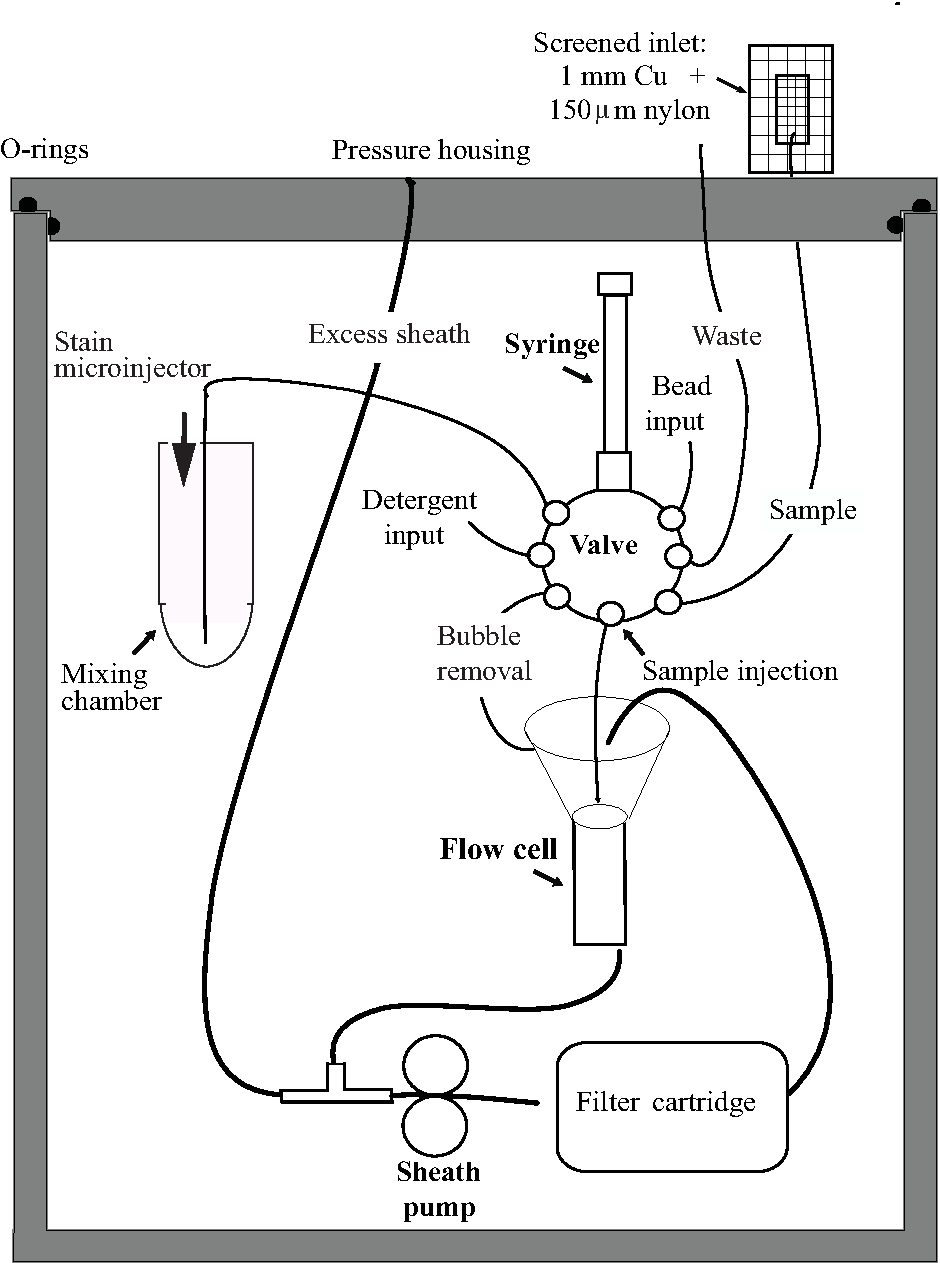
\includegraphics[scale=0.7]{fluidicsifcb5_staining_mostrecent.pdf}
\caption[Schema of fluidics for IFCB-S] {Schema of fluidics for IFCB-S showing flows for sample water
and housekeeping operations (e.g. cleaning and bubble removal) as well as the higher flow rate sheath path (distinguished by thicker lines)}
\label{arm:fig2}
\end{figure}
%\newpage


\vspace*{-3in}

\begin{figure}
%\vspace{2.4in}

\graphicspath{ {Chapter2_Figures/} }
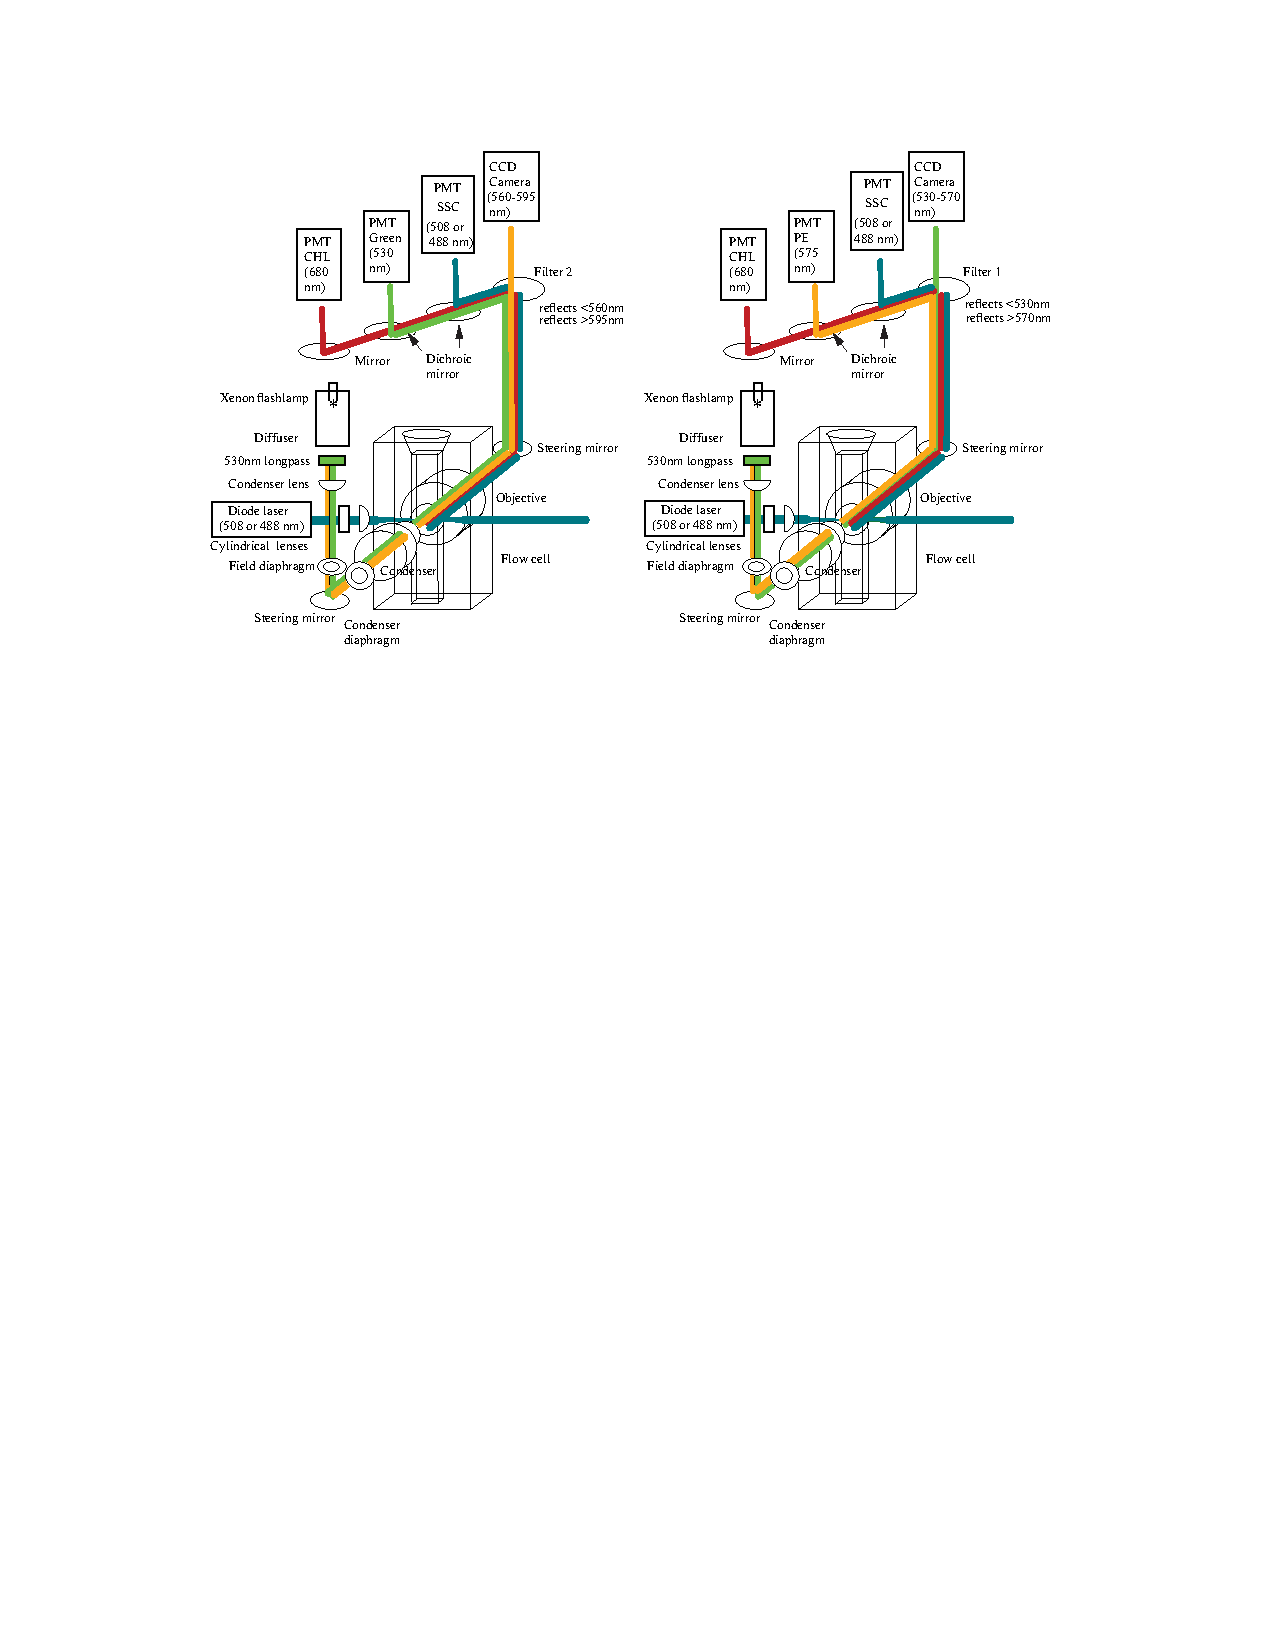
\includegraphics[scale=1, angle=90]{OpticsSchema}
\caption[Schema of optical layouts for IFCB-S in non-staining mode] {Schema of optical layouts for IFCB-S in staining mode (left panel) and non-staining mode (right panel). Both modes enable collection of chlorophyll fluorescence (CHL) and side scattering (SSC) by photomultiplier tubes (PMT). The use of filter 2 in staining mode allows detection of FDA fluorescence (Green), while the substitution of filter 1 in non-staining mode allows detection of PE fluorescence. The filter substitution results in a shift of wavelengths passed to the camera}
\label{arm:fig2}
\end{figure}

\newpage
\begin{figure}
%\vspace{2.4in}

\graphicspath{ {Chapter2_Figures/} }
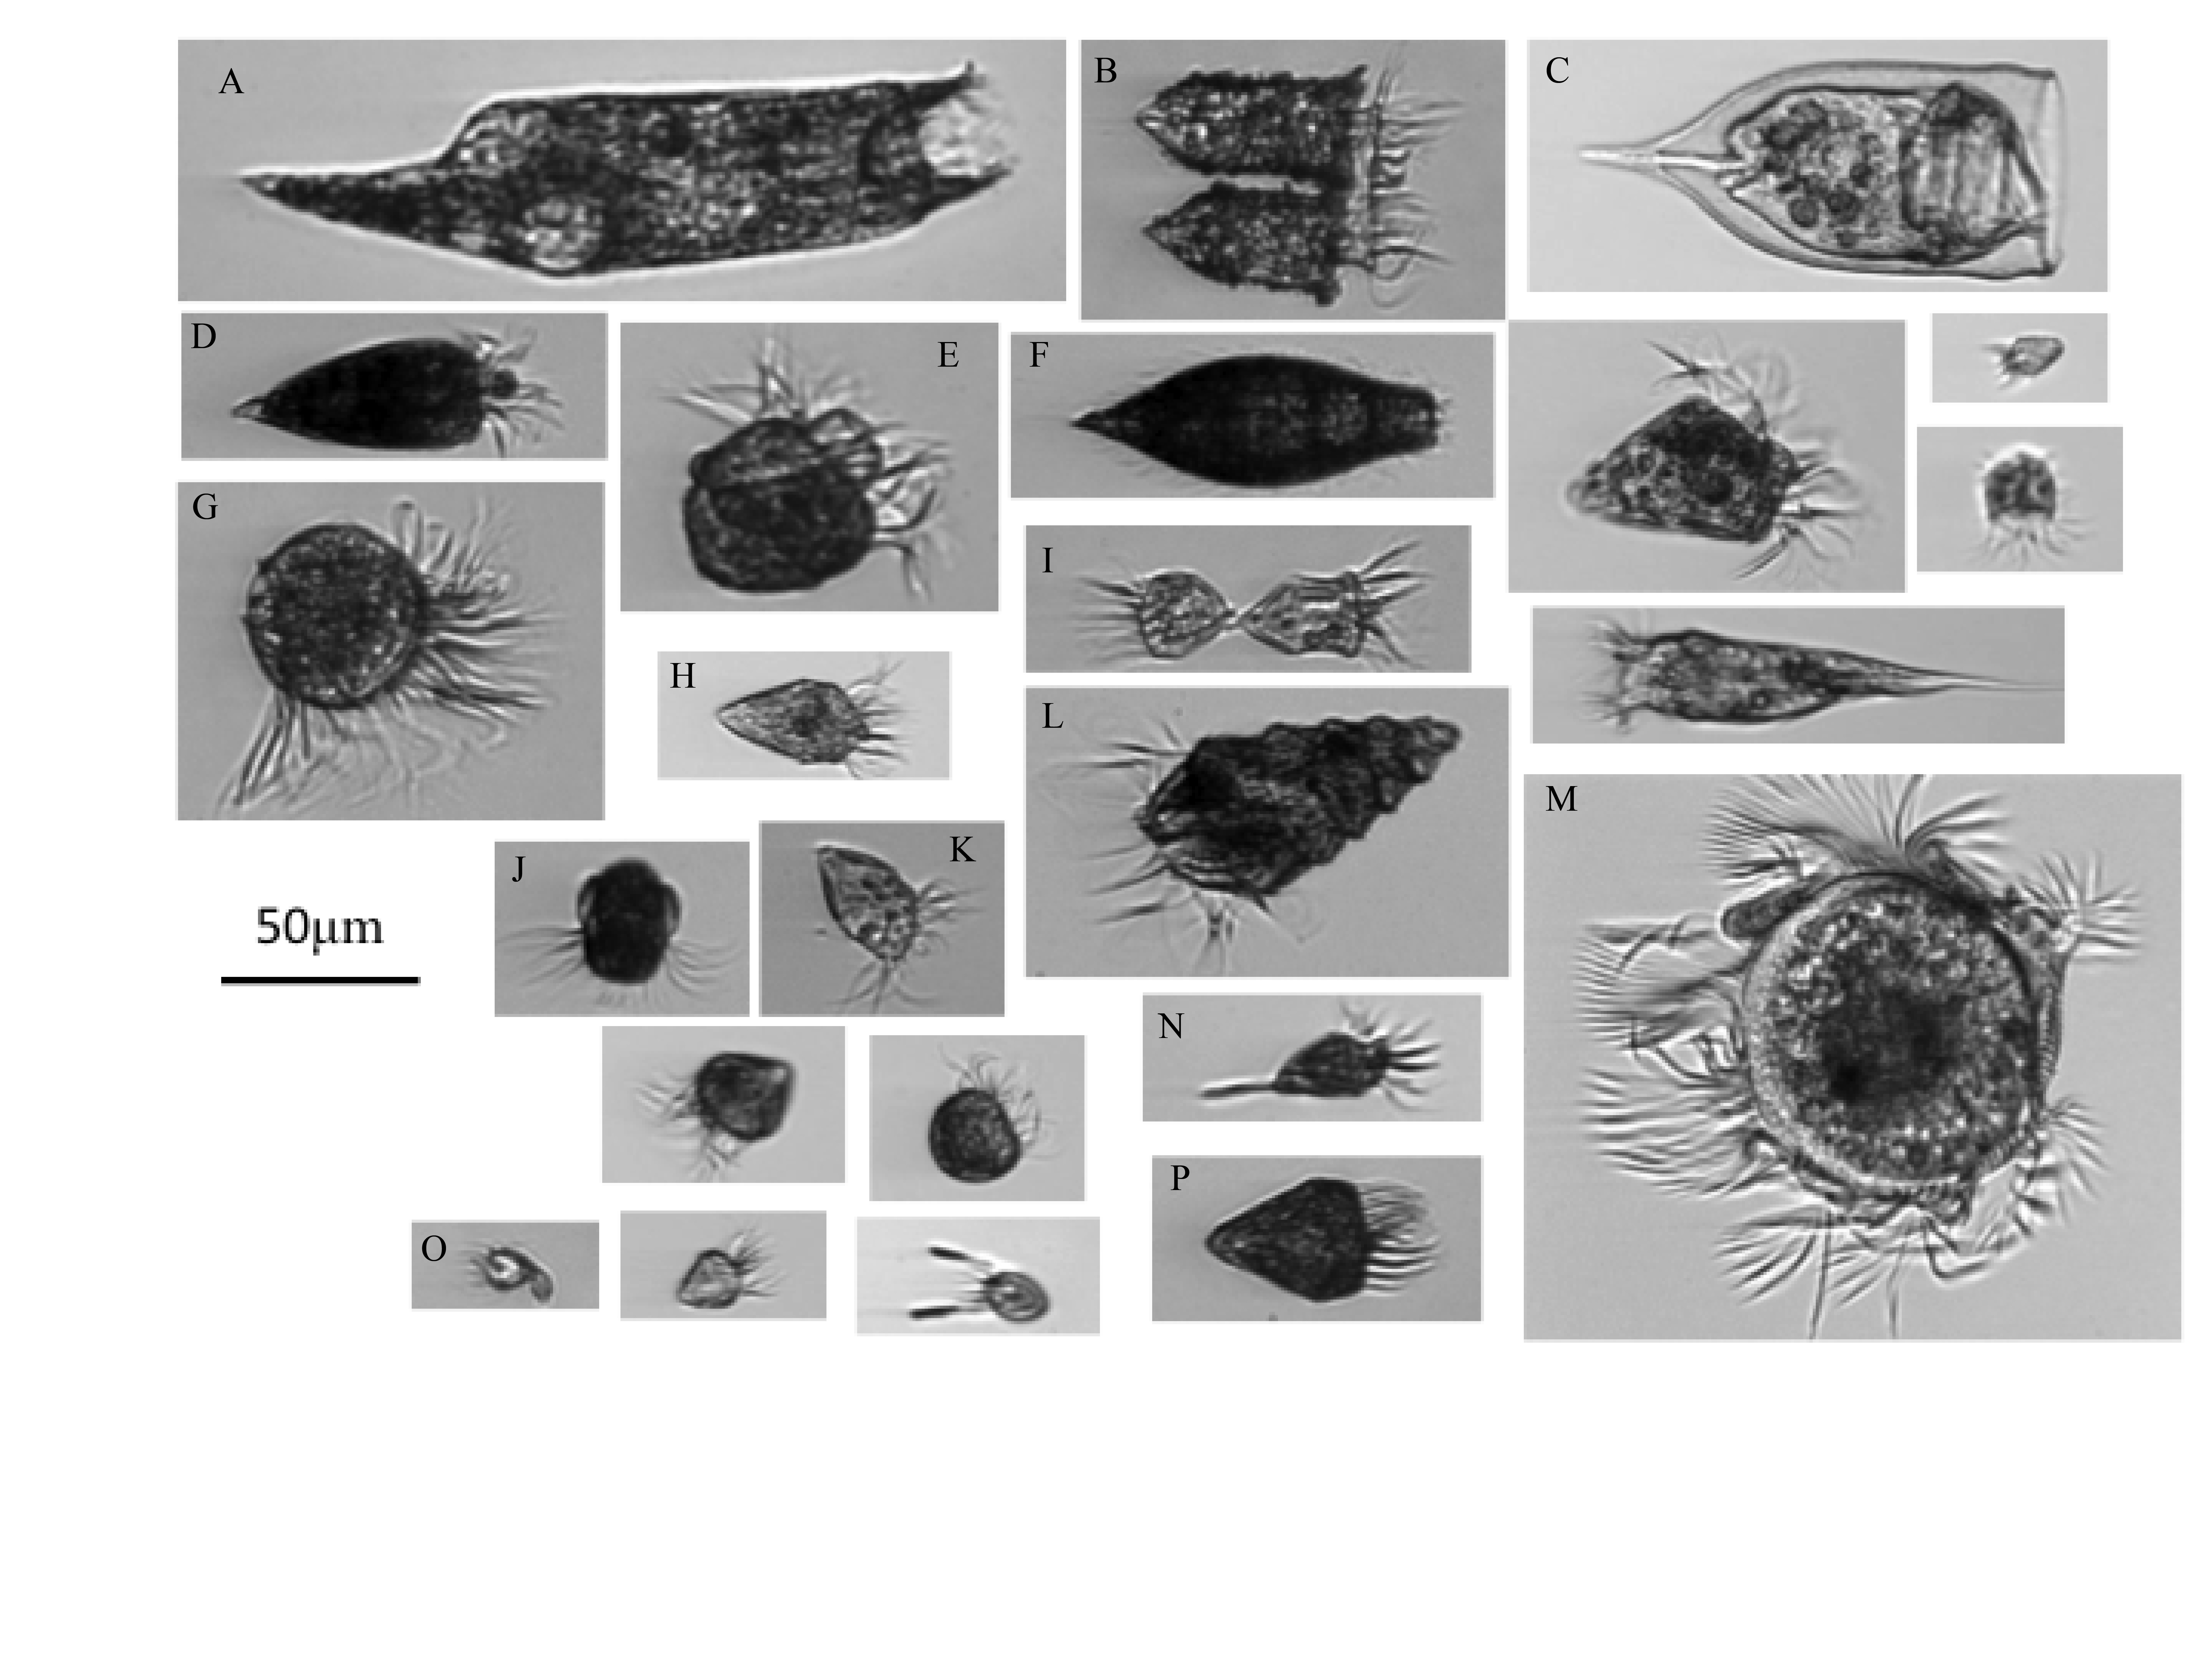
\includegraphics[scale=0.5]{MVCO_image_collage_final.jpg}
\caption [Images of ciliates at MVCO]  {Examples of ciliate categories at MVCO as imaged by standard IFCB triggering on chlorophyll fluorescence. Ciliates are grouped by similar morphology and identified to genus and species as possible. (A)\textit{Strombidium conicum}; (B \& C) tintinnid; (D) \textit{Strombidium oculatum}; (E) \textit{Strombidium capitatum}; (F) \textit{Tiarina fusus}; (G) \textit{Strobilidium} spp.; (H \& K) \textit{Strombidium} spp.; (I) \textit{Strombidium inclinatum}; (J) \textit{Mesodinium} spp.; (L) \textit{Laboea strobila}; (M) \textit{Strobilidium} spp.; (N) \textit{Pseudotontonia simplicidens}; (O) \textit{Tontonia gracillima}; (P) \textit{Strombidium} spp. The remaining categories are currently grouped together as \lq{ciliate mix}\rq because morphology is not always distinct. All images from the MVCO data set are publicly available (http://ifcb-data.whoi.edu/mvco), as is a large set of annotated ciliate images (Sosik et al. 2015)}
\label{arm:fig2}
\end{figure}

\newpage\begin{figure}
%\vspace{2.4in}

\graphicspath{ {Chapter2_Figures/} }
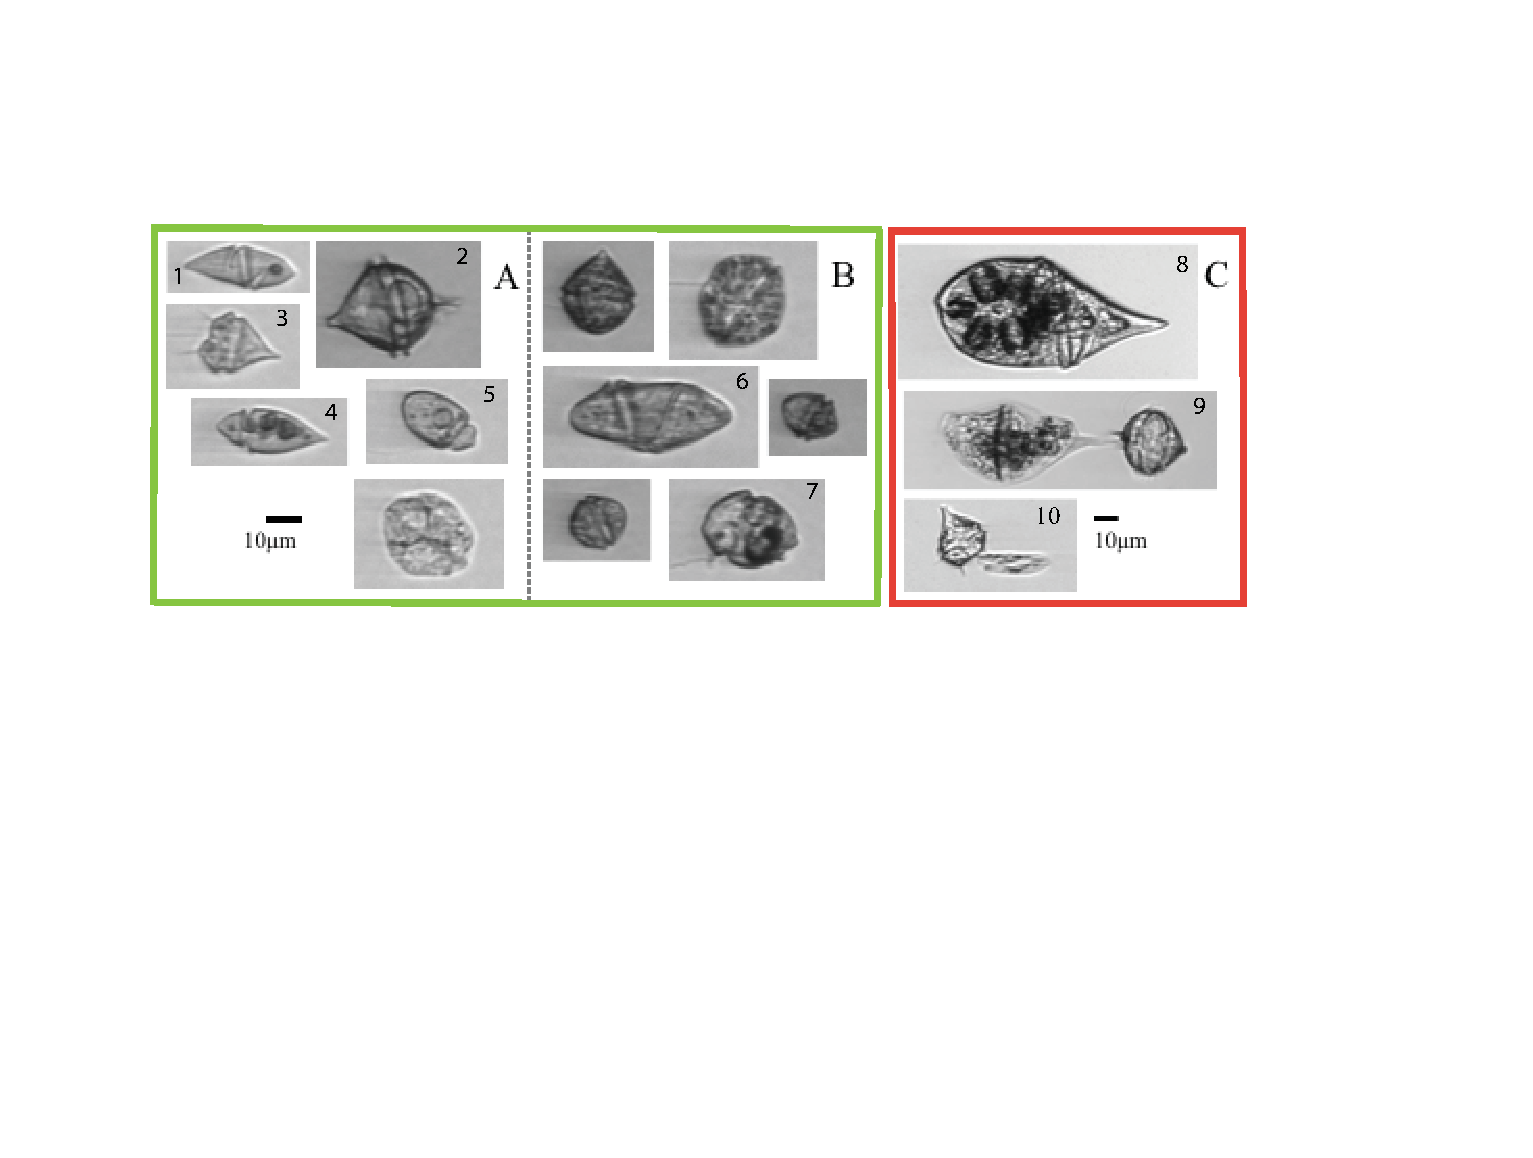
\includegraphics[scale=0.75]{dino_images}
\caption [Images of heterotrophic dinoflagellates] {Examples of dinoflagellates from Woods Hole Harbor as imaged by IFCB-S triggering on FDA and chlorophyll fluorescence (green box; A \& B) and actively grazing dinoflagellates at MVCO as imaged by a standard IFCB triggering on chlorophyll
fluorescence (red box; C). (A) Dinoflagellates with low chlorophyll and high stain fluorescence; (B) dinoflagellates with both high chlorophyll and stain fluorescence. Some categories are grouped by morphology, others have been identified to genus level: gyrodinoid dinoflagellate (1, 6, 8); \textit{Protoperidinium} spp. (2, 9), \textit{Protoperidinium} spp. (3, 10); \textit{Amphidinium} spp.
(4, 5); \textit{Proterythropsis} spp. (7). The unnumbered examples are currently grouped together in our classification }
\label{arm:fig2}
\end{figure}

\begin{figure}
%\vspace{2.4in}

\graphicspath{ {Chapter2_Figures/} }
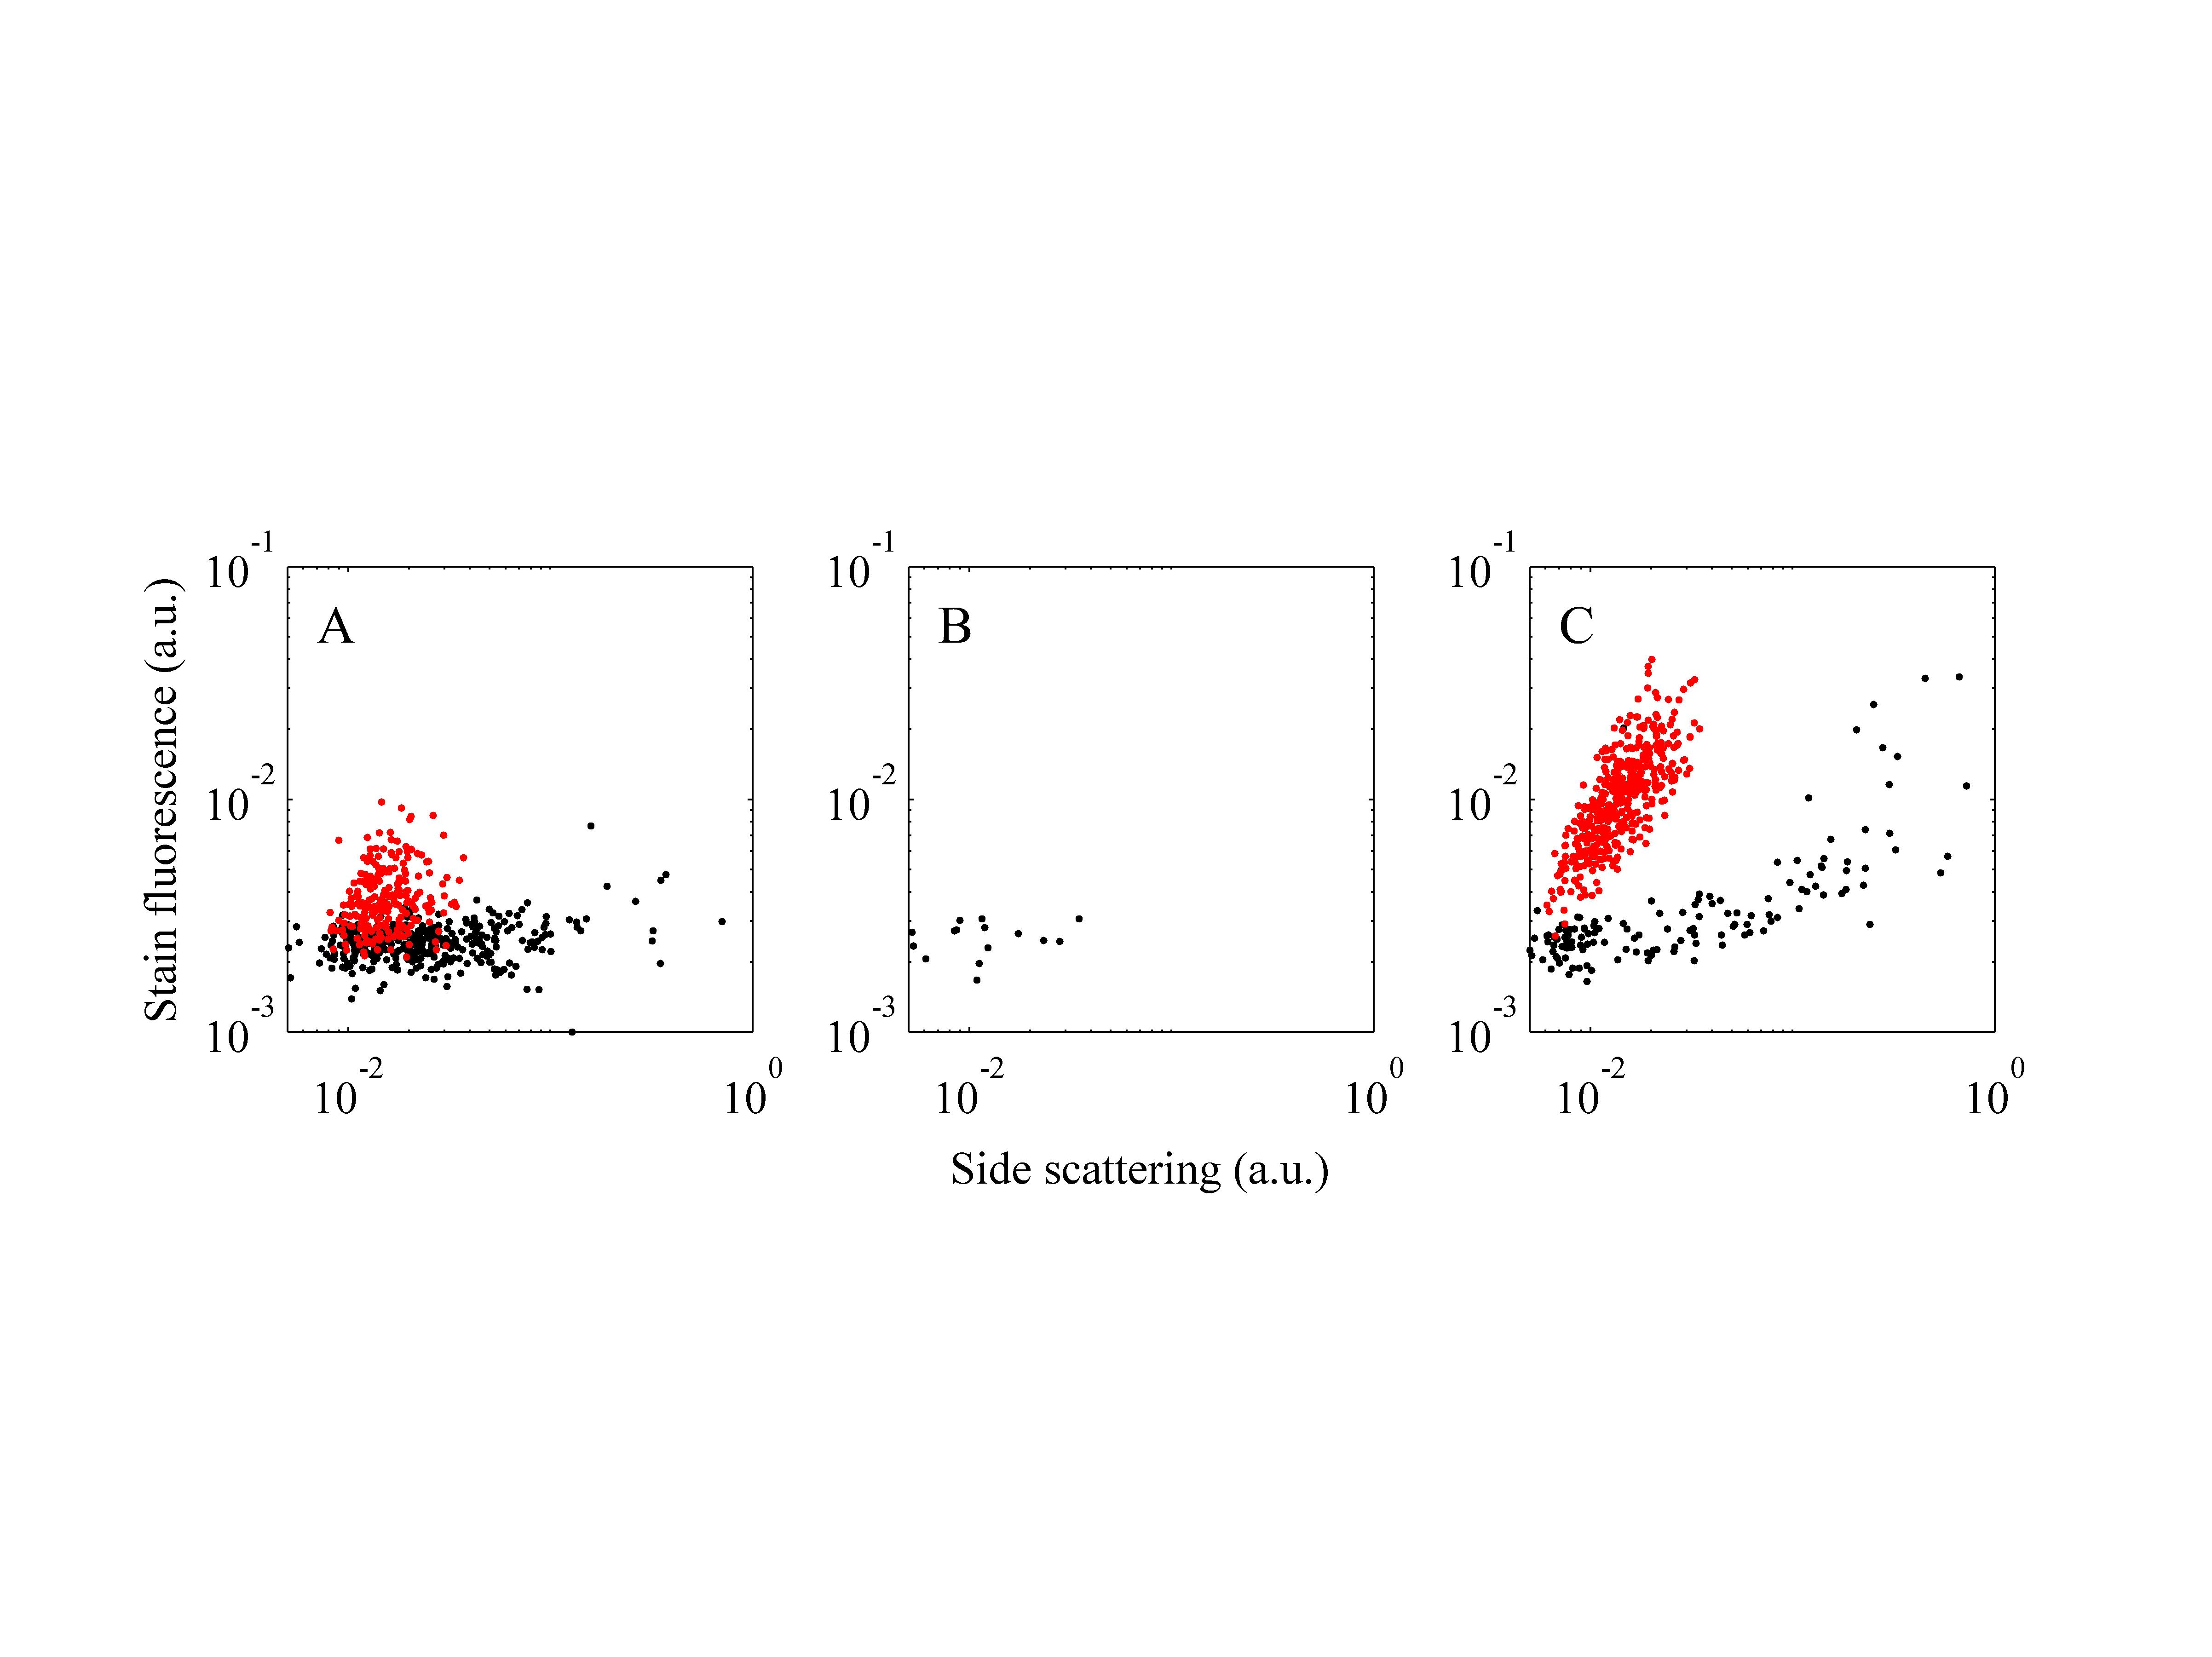
\includegraphics[scale=0.1]{scut_protocol_testing_au}
\caption [FDA staining validation] {Relationship between FDA fluorescence and side angle light scattering (integrated signals) for subsamples of a scuticociliate culture analyzed with IFCB-S configured in different triggering modes. (A) Unstained sample with triggering on side scattering; (B) unstained sample with triggering on stain fluorescence; (C) stained sample triggering on stain fluorescence. Black dots indicate detrital particles and red dots are scuticociliates, as determined from visual inspection of associated images. a.u.: arbitrary units}
\label{arm:fig2}
\end{figure}

\begin{figure}
%\vspace{2.4in}

\graphicspath{ {Chapter2_Figures/} }
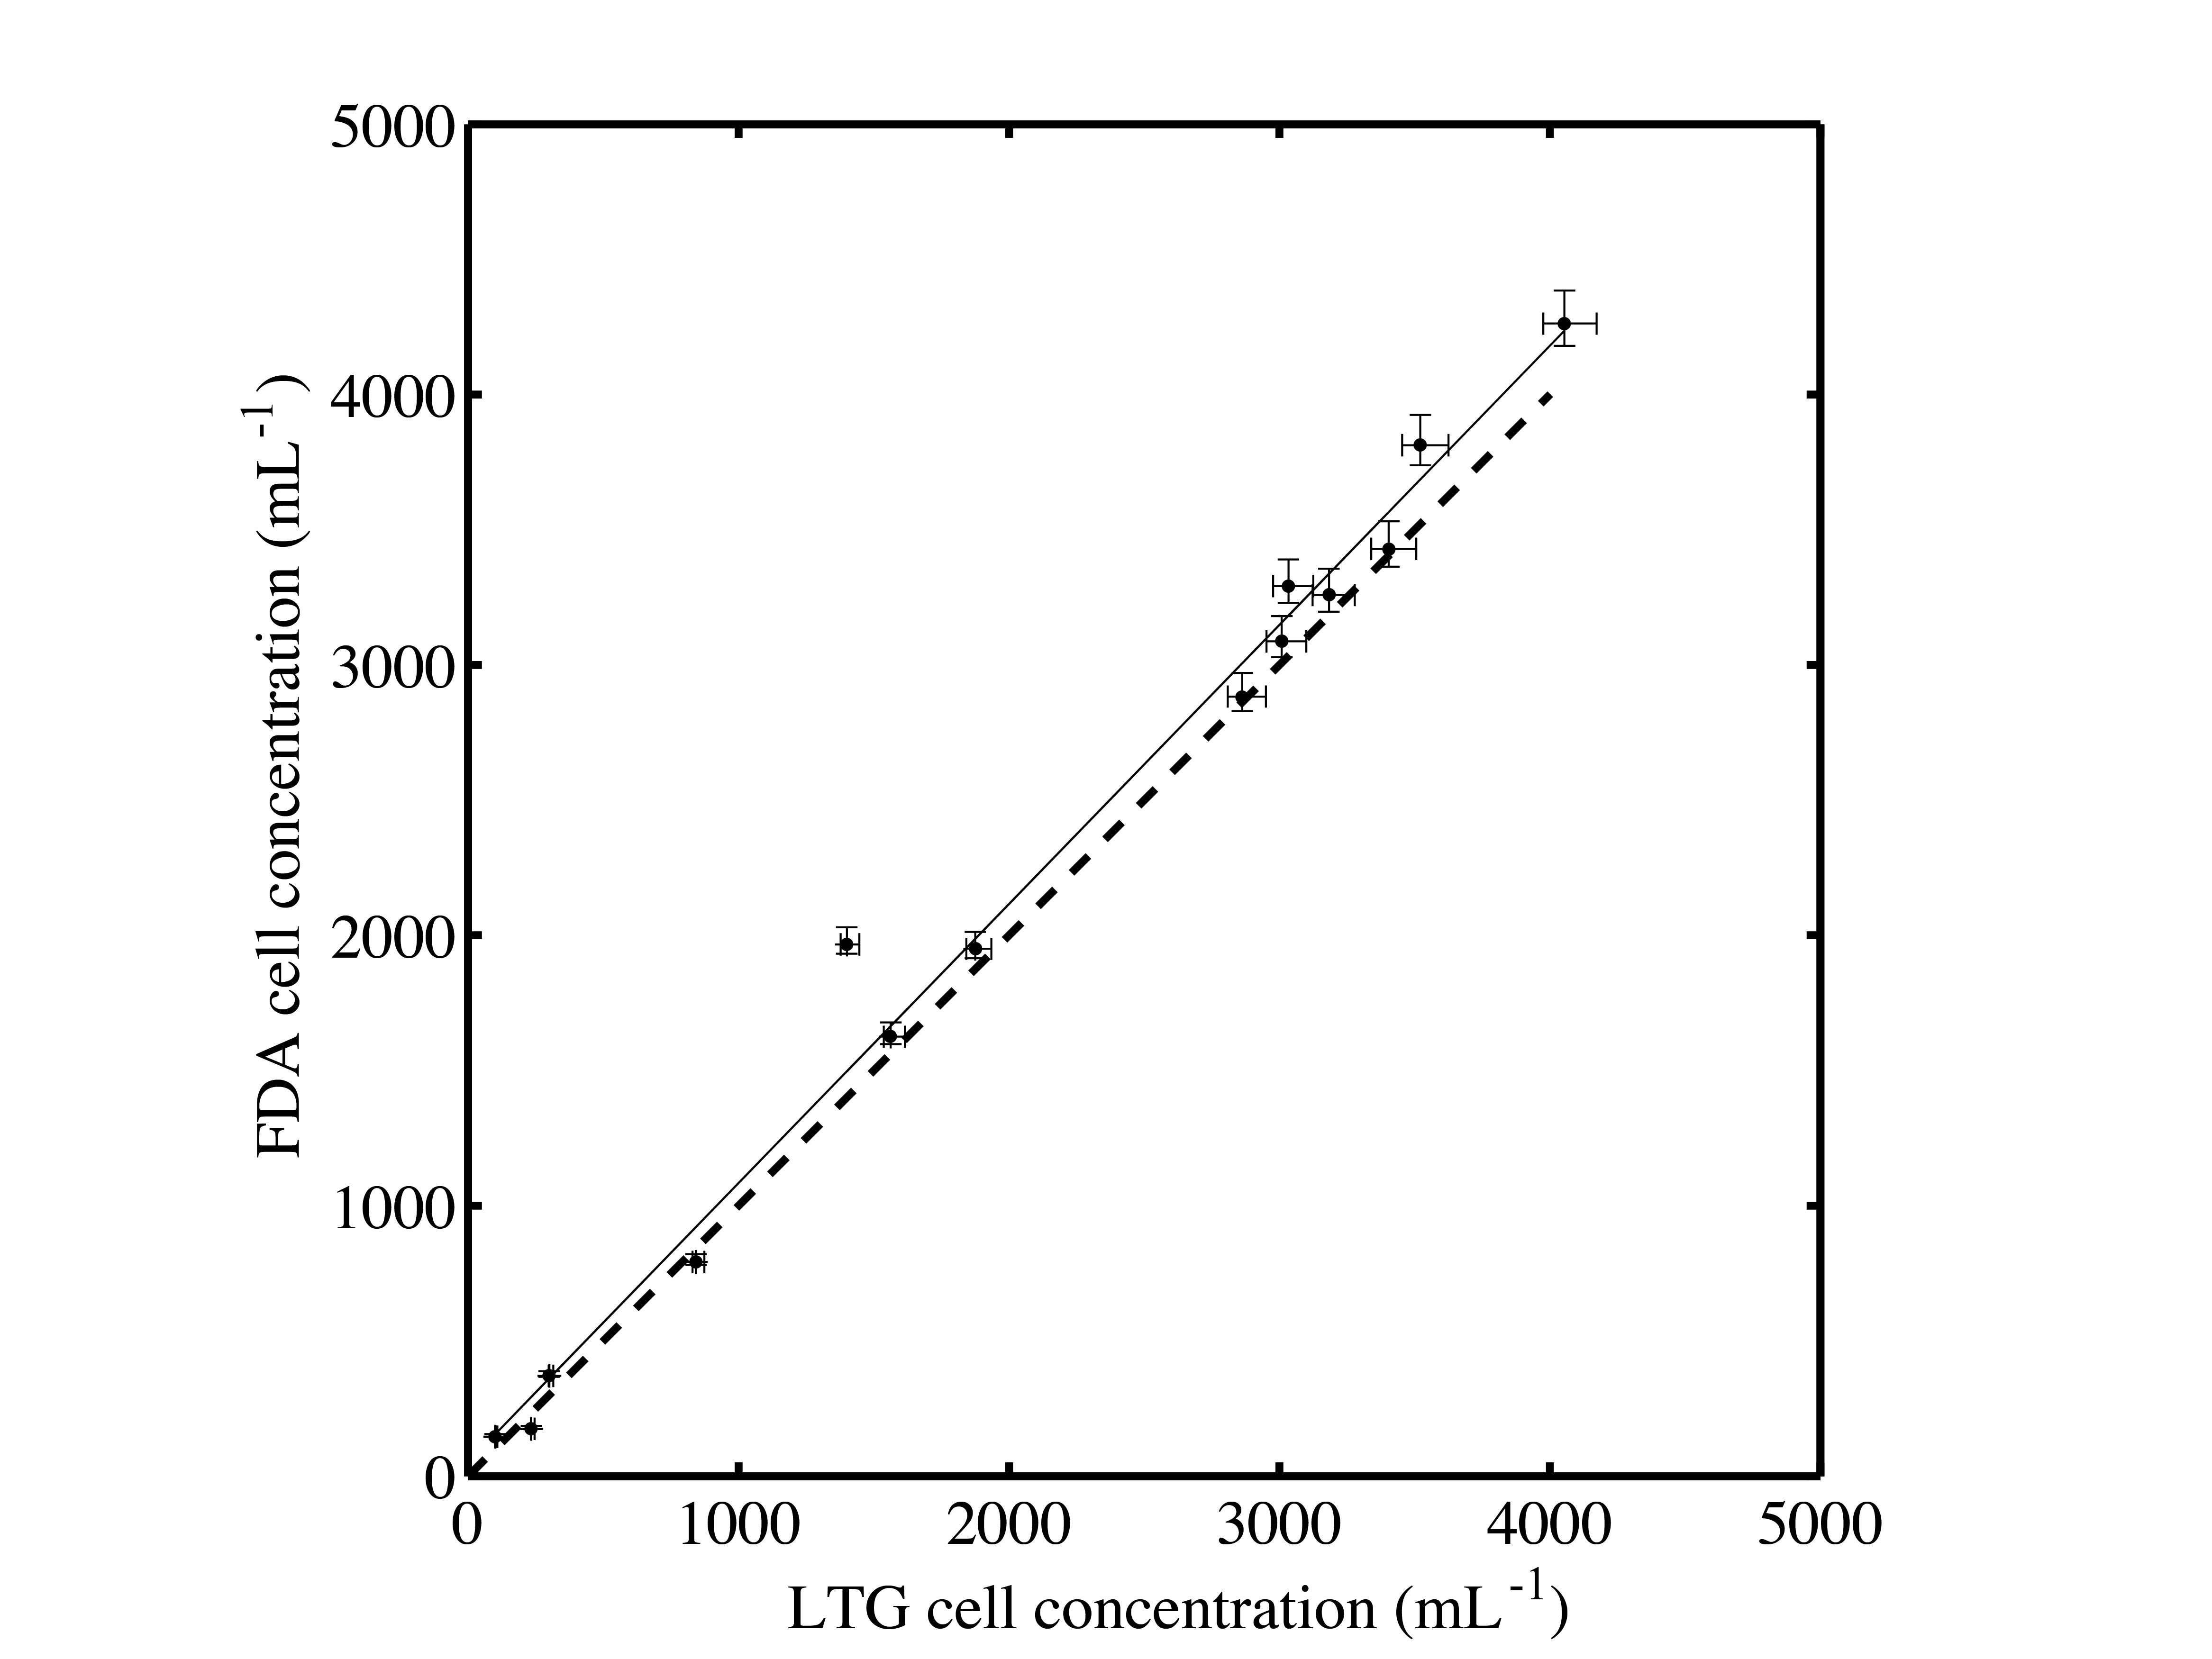
\includegraphics[scale=0.1]{FDA_vs_LTG_mostrecent}
\caption [Comparison between FDA and LTG] {Comparison of flow cytometric detection of a scuticociliate culture stained with FDA or LTG. Solid line is best fit. Dashed line is 1:1. 95\% confidence intervals are shown for each count}
\label{arm:fig2}
\end{figure}

\newpage
\begin{figure}
%\vspace{2.4in}

\graphicspath{ {Chapter2_Figures/} }
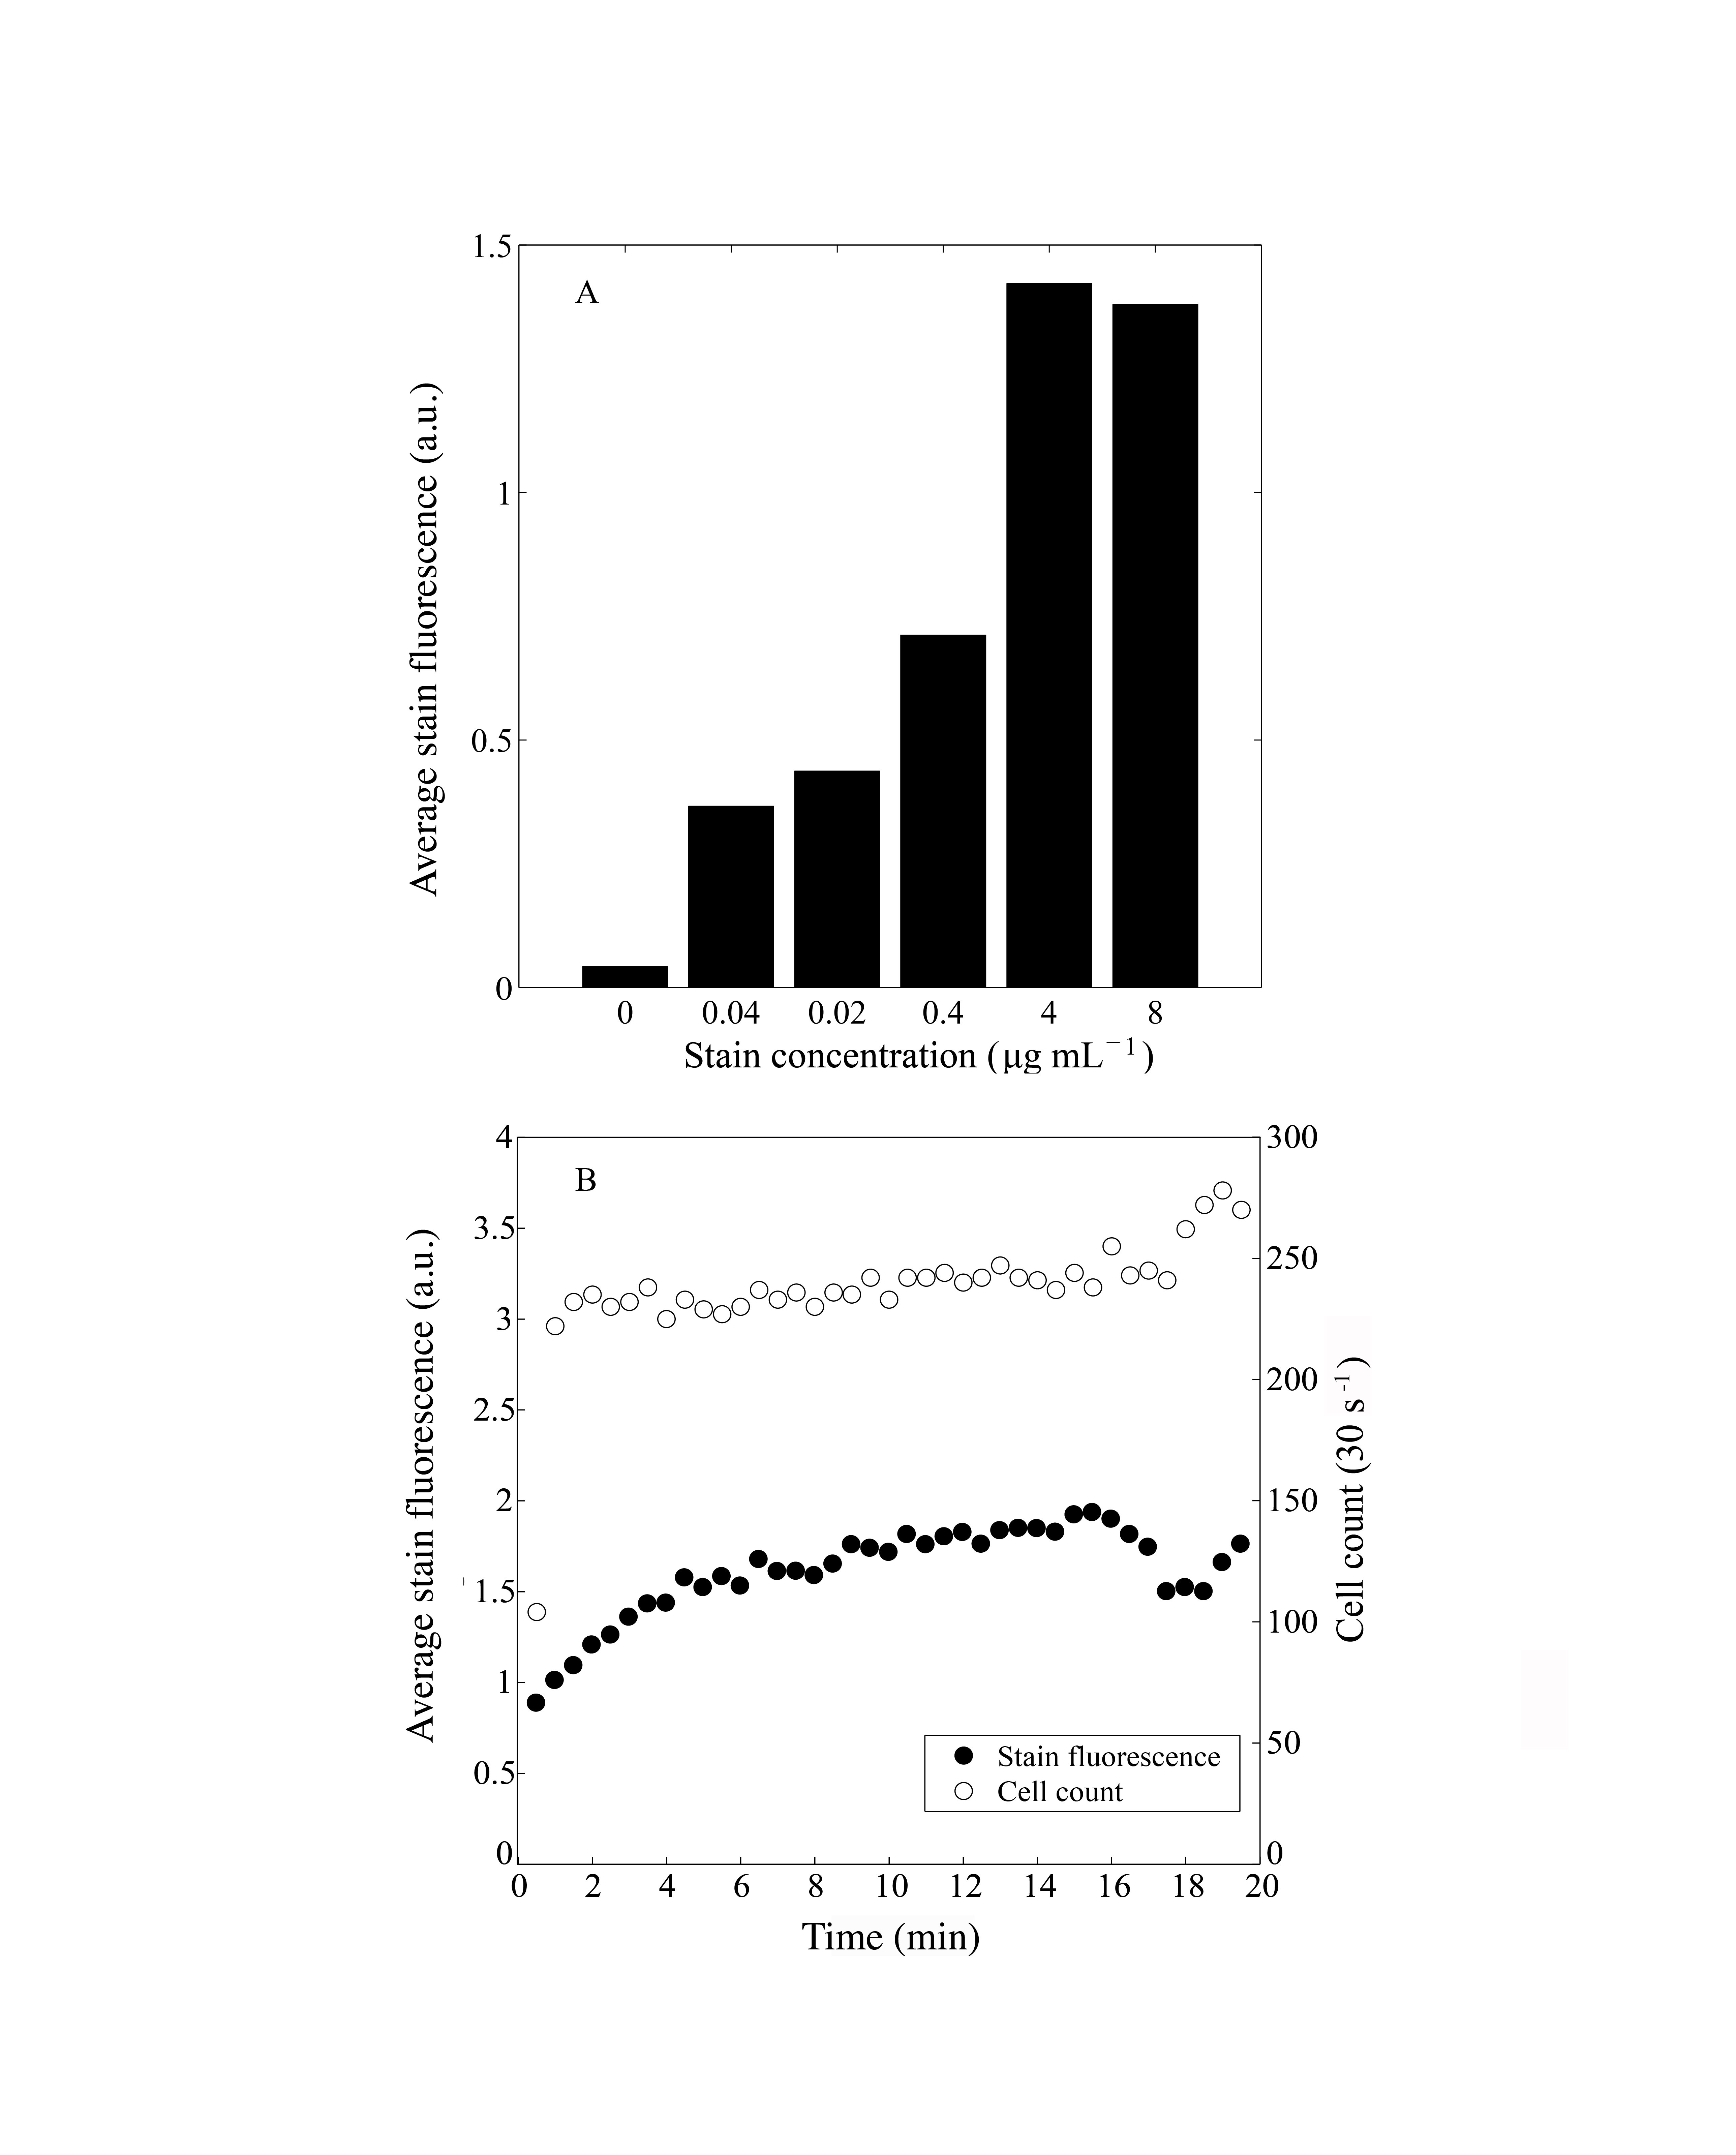
\includegraphics[scale=0.7]{Final_stain_tests_au}
\caption [Testing stain protocol] {(A) Average stain fluorescence values of cells from a scuticociliate culture incubated with a range of final FDA stain concentration. Unstained sample (0 $\upmu$g FDA ml$^{-1}$) was triggered on scattering. (B) Average stain fluorescence values and scuticociliate cell counts within 30 s bins during 20 min analysis of one 5 ml sample. Open circles and closed circles represent whole cell counts and average stain fluorescence, respectively }
\label{arm:fig2}
\end{figure}

\begin{figure}
%\vspace{2.4in}

\graphicspath{ {Chapter2_Figures/} }
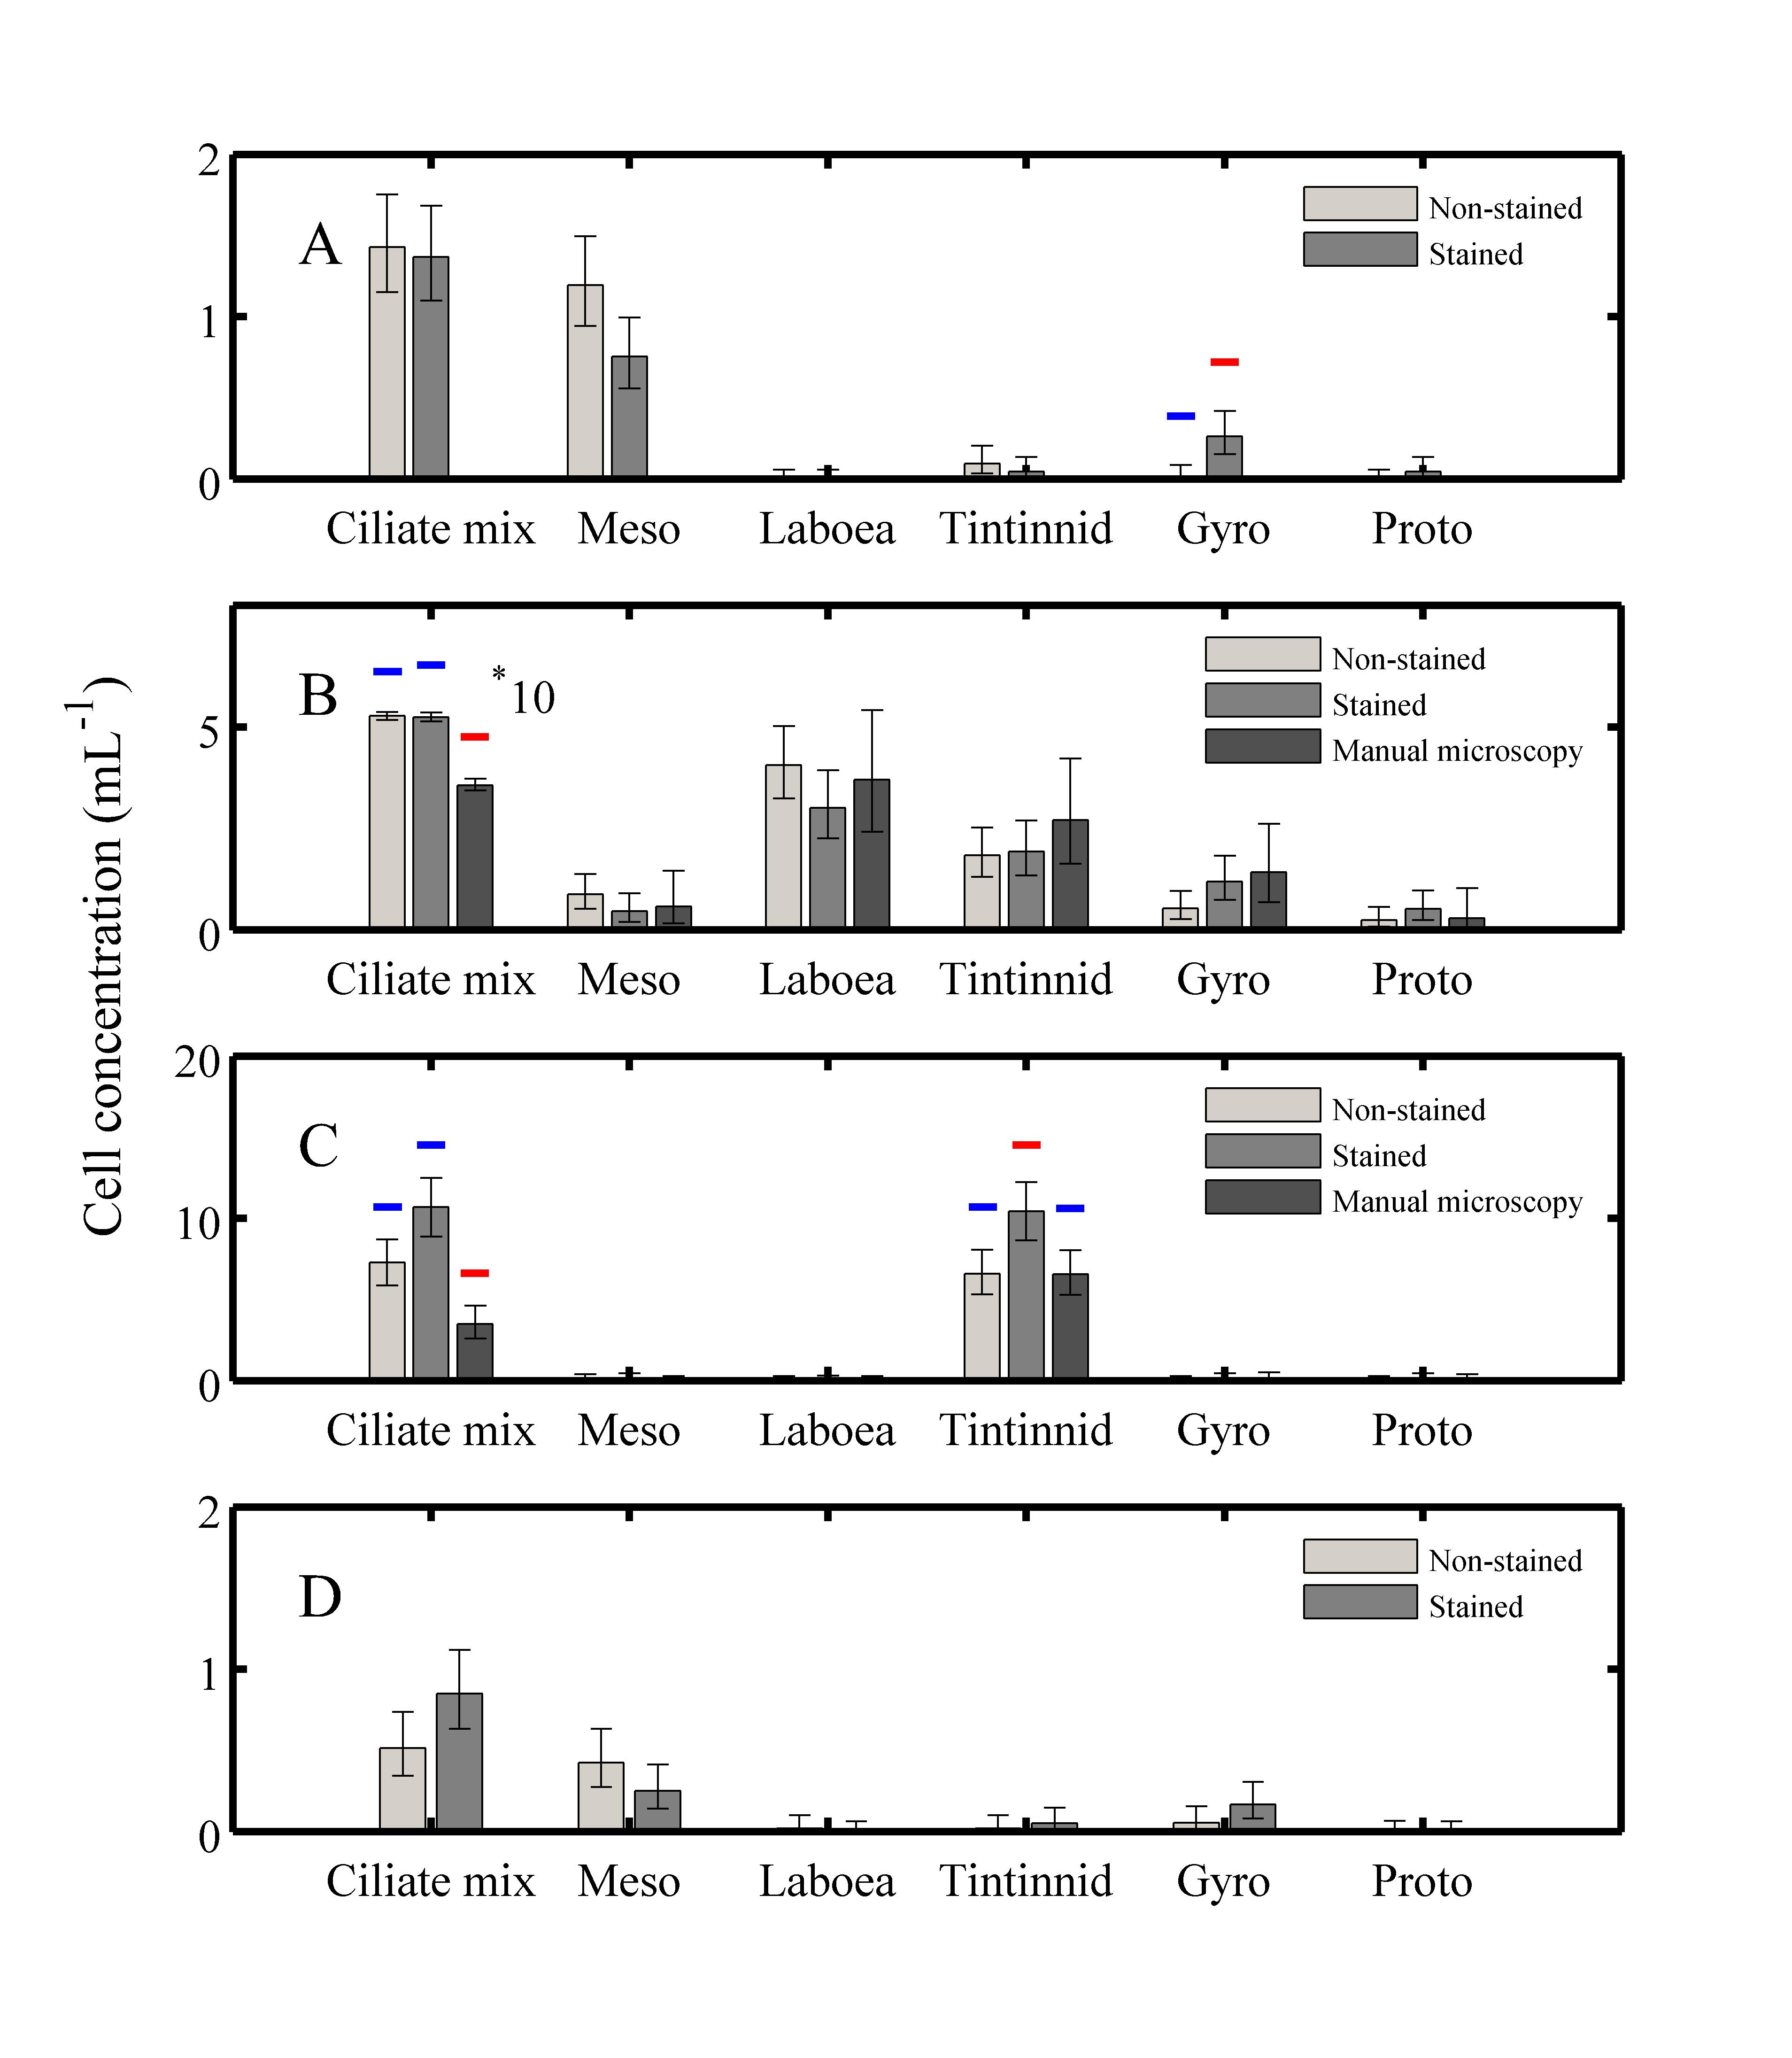
\includegraphics[scale=0.1]{seasonal_comparison}
\caption [Seasonal comparisons between manual microscopy and IFCB-S] {Cell concentrations (cells ml$^{-1}$) for ciliate mix, \textit{Mesodinium} spp., \textit{Laboea strobila}, tintinnids, \textit{Gyrodinium} spp., and \textit{Protoperidinium} spp. comparing results from manual microscopy with samples analyzed by IFCB-S operated in staining and nonstaining modes. Samples were collected from Woods Hole Harbor in winter (A: January 19, 2014), spring (B: May 11, 2014), summer (C; July 2, 2014), and fall (D; October 18, 2014), with manual microscopy only available for winter and fall. Error bars indicate 95\% confidence intervals computed assuming Poisson distributed counting statistics. Significance is indicated by colored bars; red and blue bars are significantly different from each other. If no significant differences were found within a taxonomic group, no bars are displayed. Total cell counts for winter, spring, summer, and fall range from 0 to 89, 8 to 250, 0 to 132, and 0 to 51, respectively)}
\label{arm:fig2}
\end{figure}

\begin{figure}
%\vspace{2.4in}

\graphicspath{ {Chapter2_Figures/} }
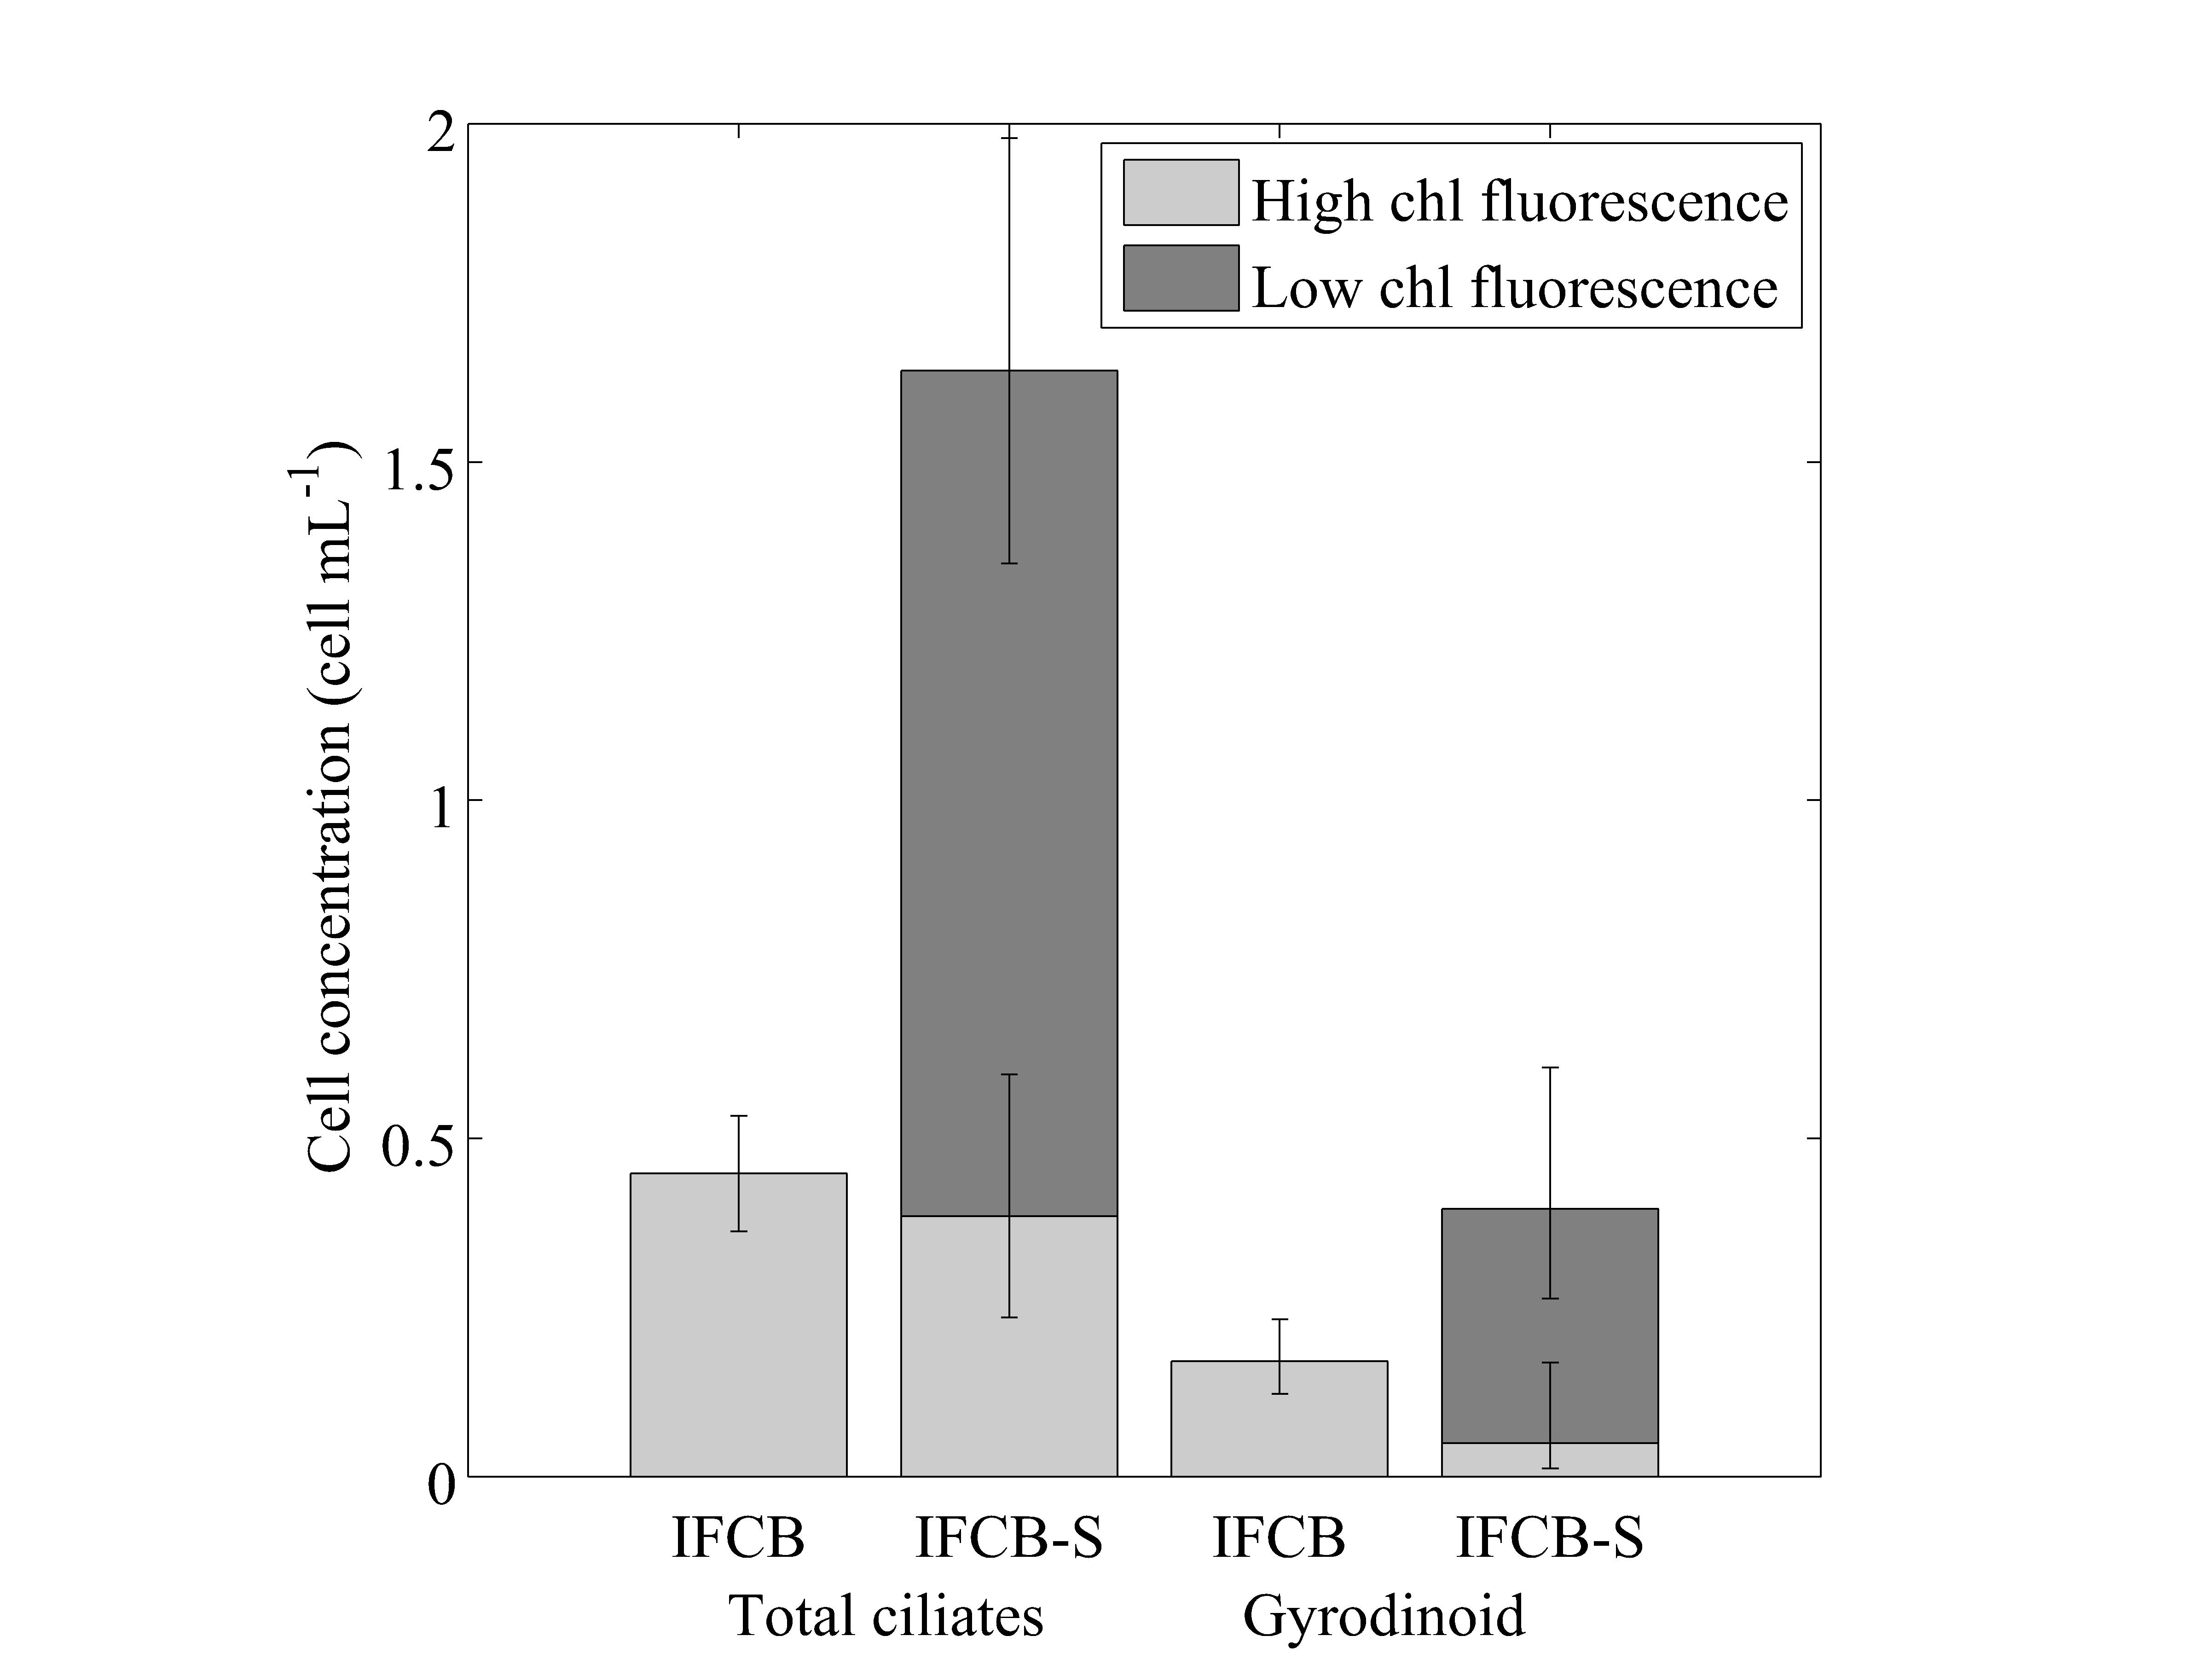
\includegraphics[scale=0.1]{OKEX_staining_updated}
\caption [OKEX cruise comparison between staining and non-staining on IFCB-S] {Daily-binned cell concentration for total ciliates and gyrodinoid dinoflagellates imaged on August 25, 2014, during the ECOMON cruise. Light and dark grey bars indicate populations with high and low chlorophyll fluorescence, respectively. Error bars indicate 95\% confidence intervals computed assuming Poisson distributed counting statistics.}
\label{arm:fig2}
\end{figure}

\newpage
\begin{figure}
%\vspace{2.4in}

\graphicspath{ {Chapter2_Figures/} }
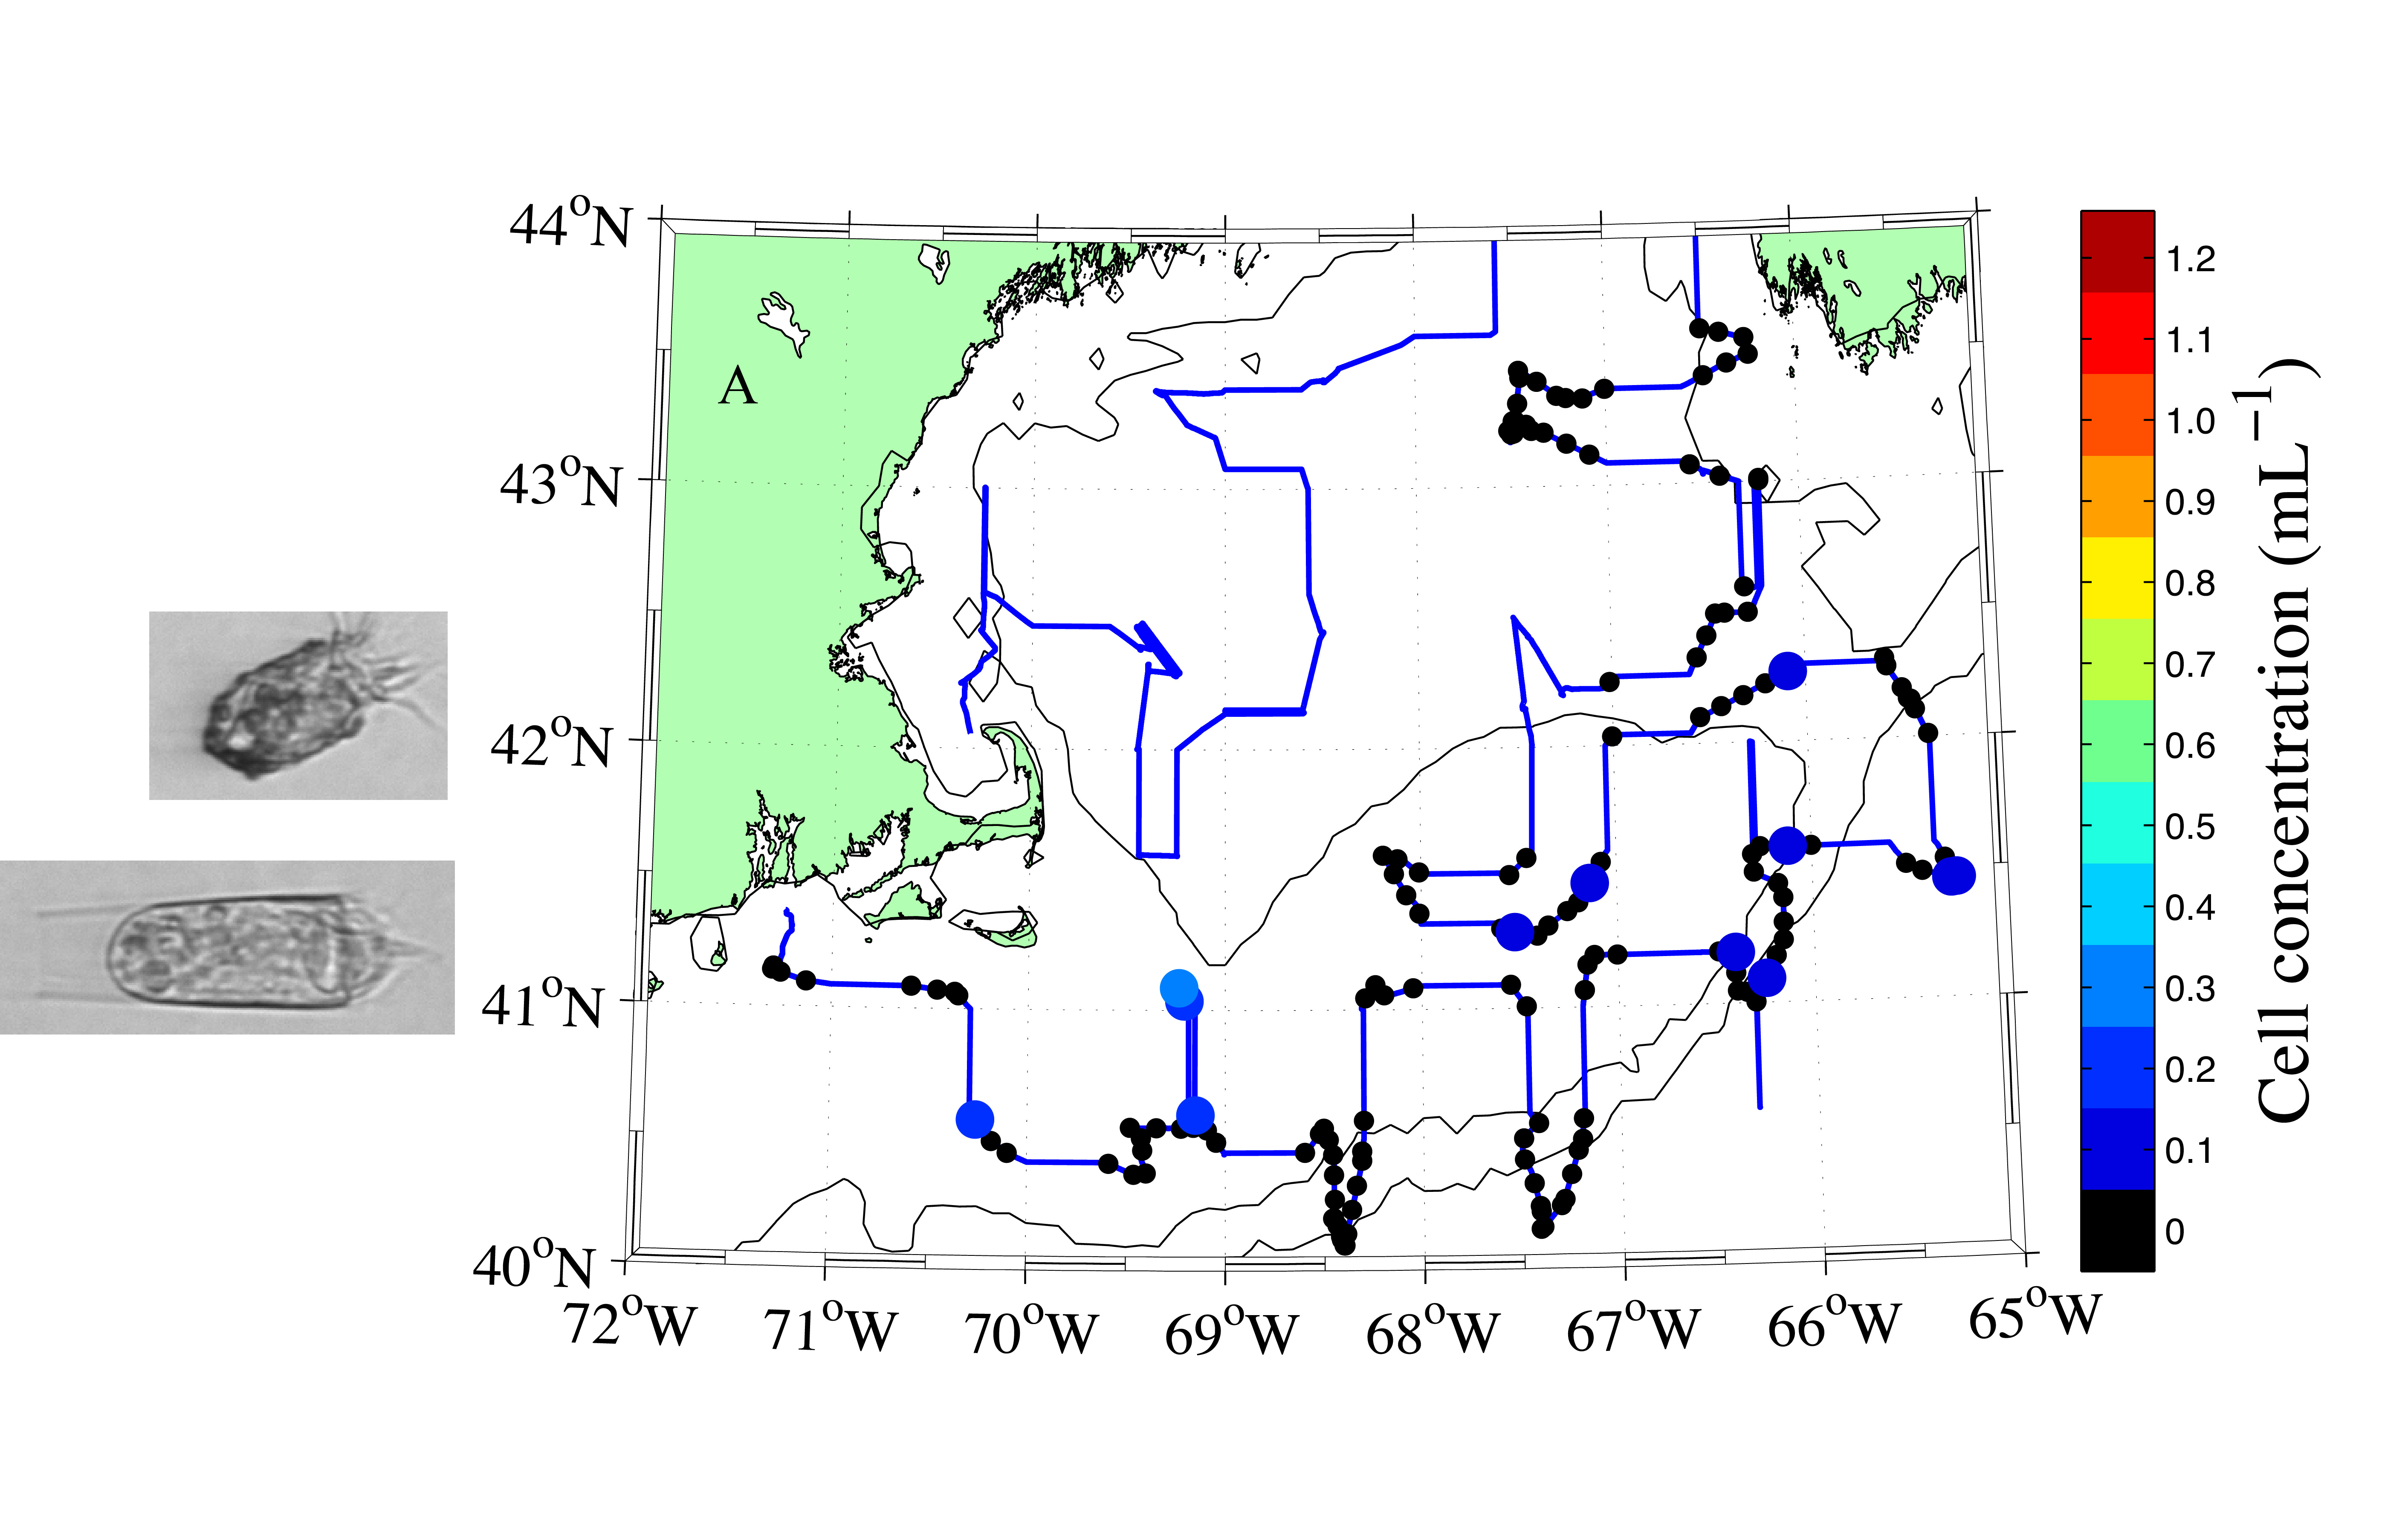
\includegraphics[scale=0.5]{normal_map_fixedcolorbar_most_recent}
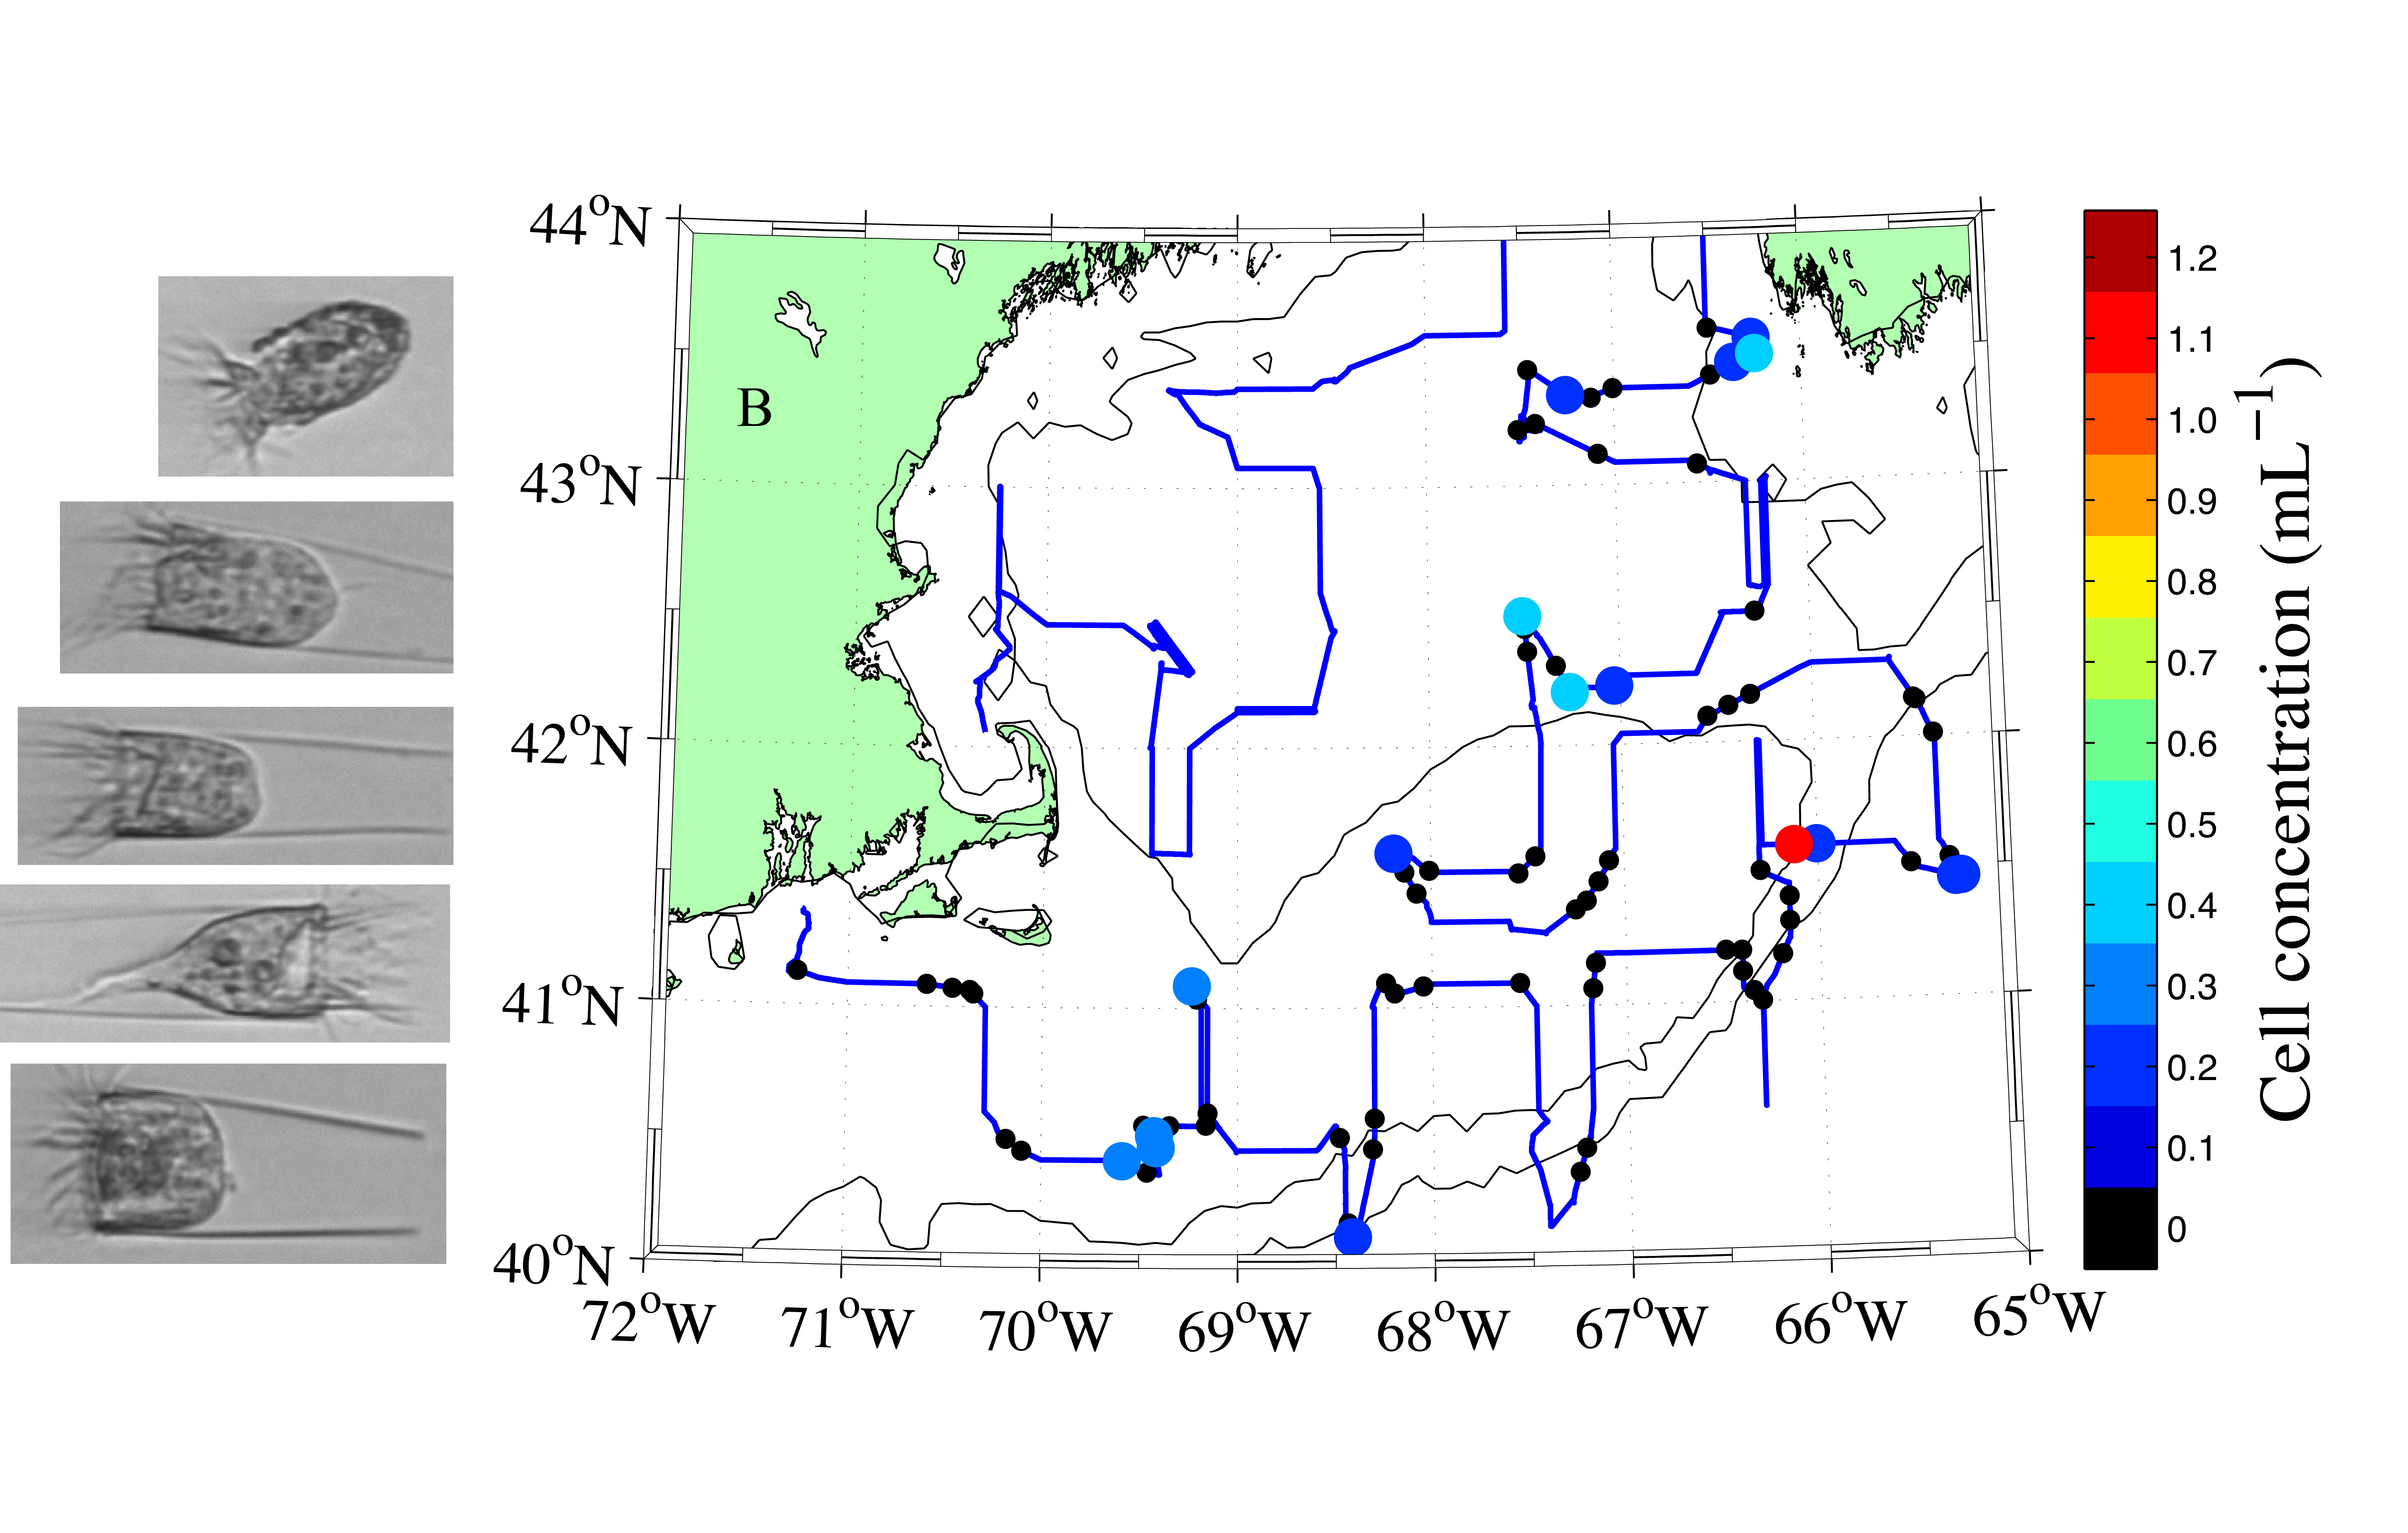
\includegraphics[scale=0.5]{alt_map_fixedcolorbar_most_recent}
\caption [Tintinnid abundances observed on OKEX cruise between IFCB-S and a standard IFCB] {Concentration of tintinnids observed during hourly intervals in surface waters along the ECOMON cruise track in August-September 2013. Black symbols indicate locations where no tintinnids were observed. (A) Abundances observed with a standard IFCB. (B) Abundances observed with IFCB-S. Example images found around the tintinnid hotspot (station with $\sim$1.1 ml$^{-1}$ on lower map) are shown to the left of each map, with approximate frequency distribution of the observed morphotypes reflected in the examples shown. Hyaline morphotype (distinguished by transparent lorica) is \textit{Eutintinnus} spp; agglomerated morphotype is \textit{Tintinnopsis} spp.}
\label{arm:fig2}
\end{figure}

\begin{figure}
%\vspace{2.4in}

\graphicspath{ {Chapter2_Figures/} }
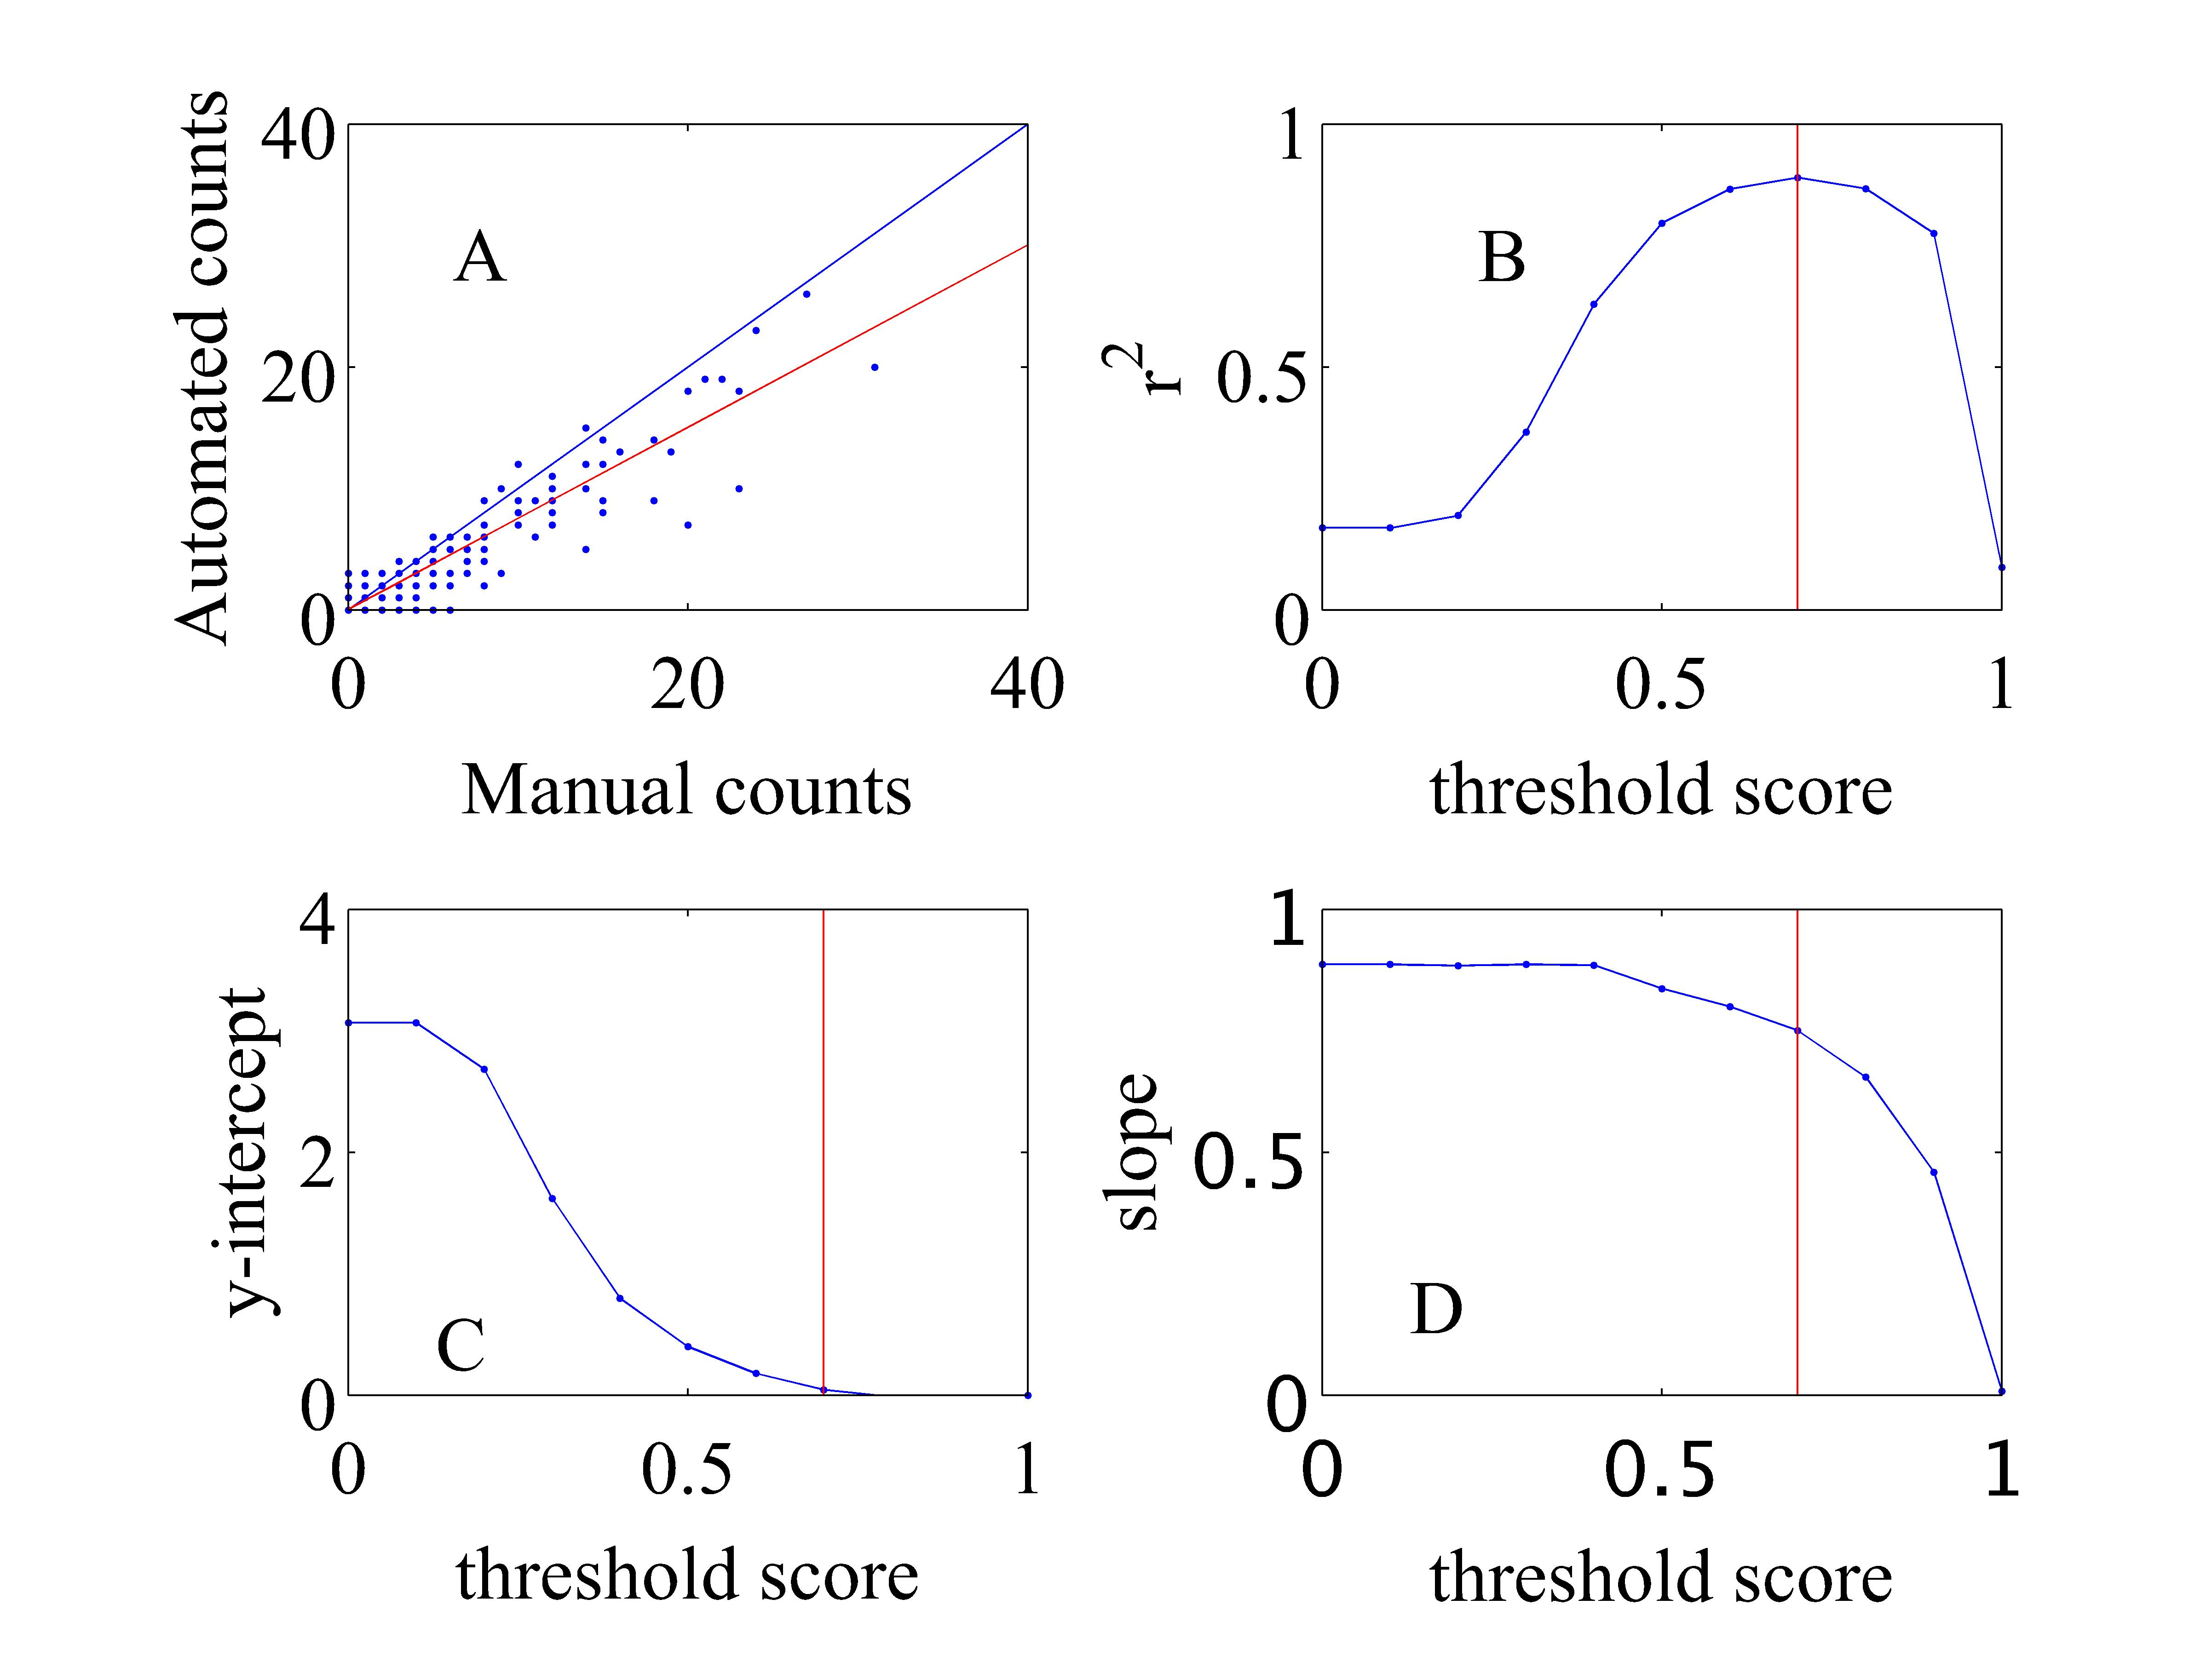
\includegraphics[scale=0.1]{threshold_summary}
\caption [ Indicators for optimal threshold use in automated classification] {(A) Regression between hourly bins of manually identified  \textit{Laboea strobila} cell abundances at MVCO and automated
classification results for score threshold 0.7. The blue line represents a 1:1 line and the red line is best fit; (B) R$^{2}$ values for all thresholds tested; (C) y-intercept values of best fit line for all thresholds tested; (D) slope values of best fit line for all thresholds tested. Vertical green line in B-D indicates selected threshold score of 0.7}
\label{arm:fig2}
\end{figure}

\begin{figure}
%\vspace{2.4in}

\graphicspath{ {Chapter2_Figures/} }
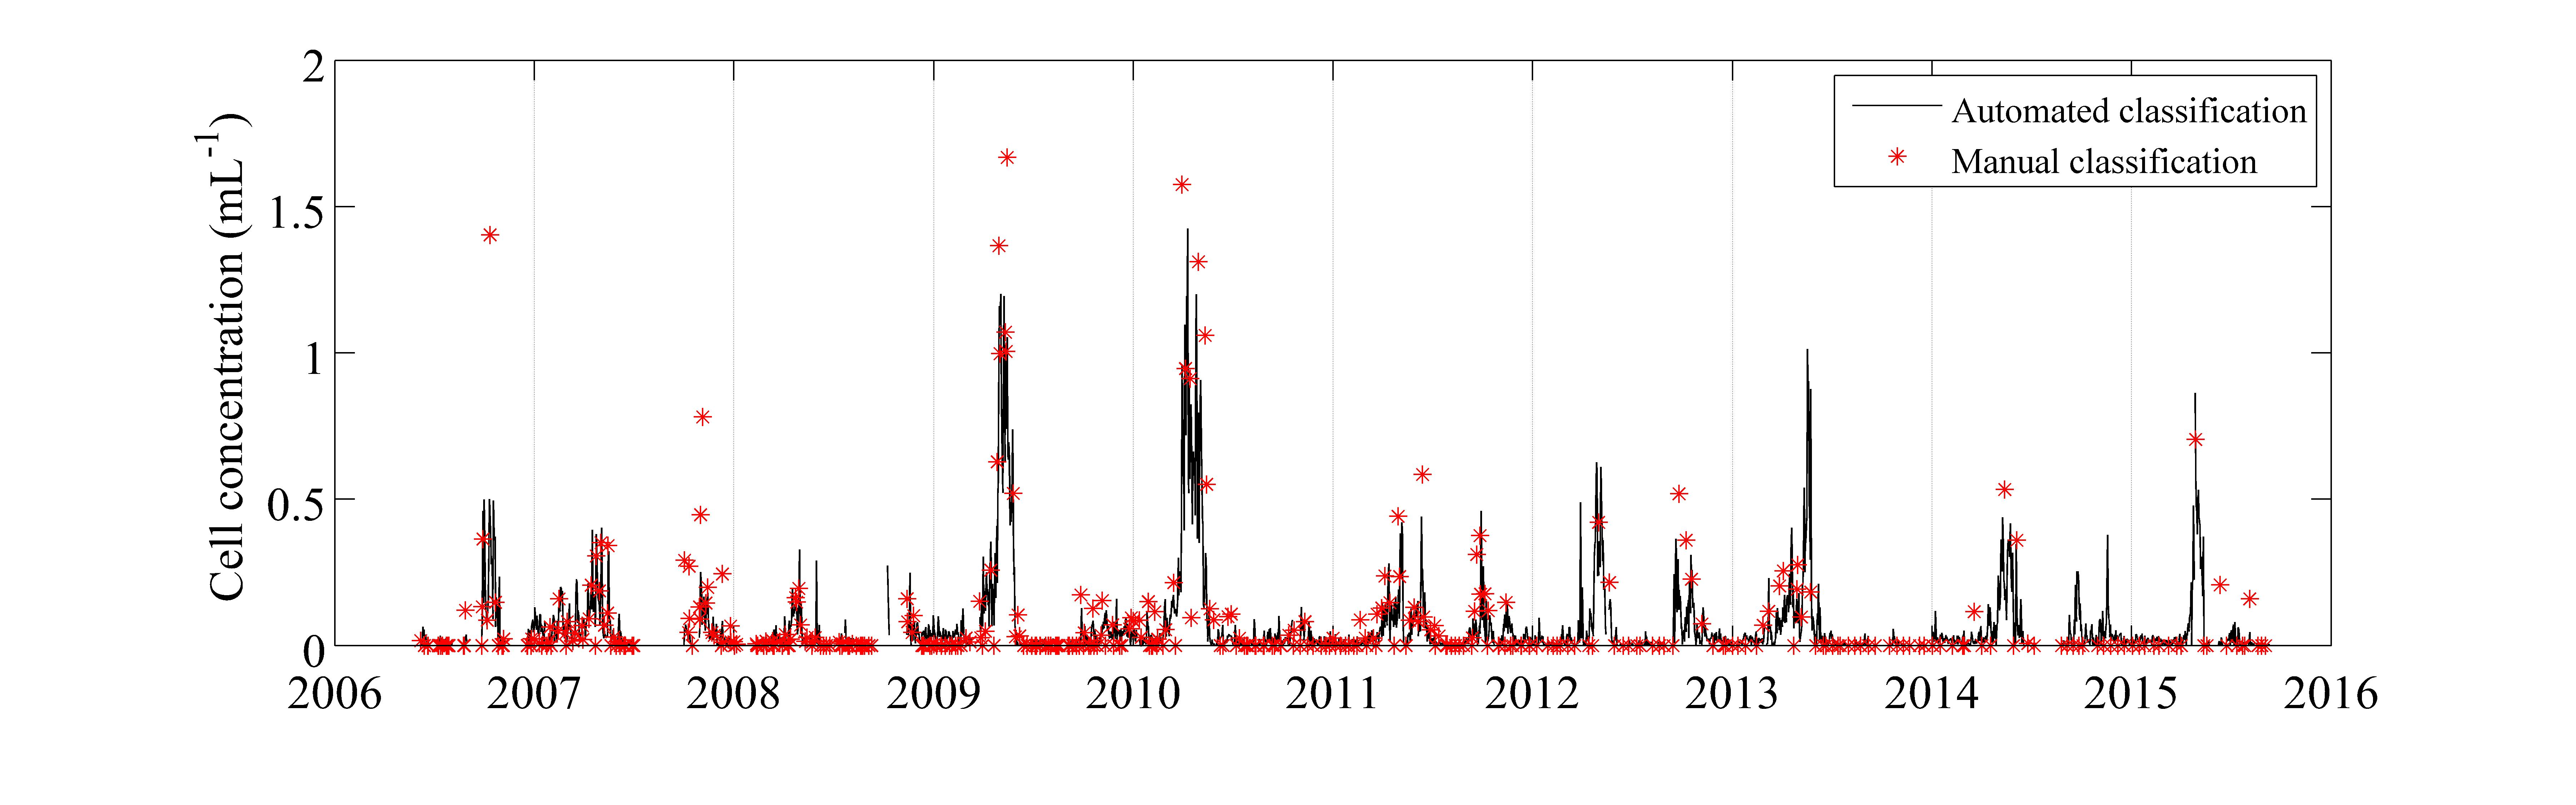
\includegraphics[scale=0.07, angle=90]{laboea_tb_updated}
\caption [Comparison between automated and manual classification for \textit{Laboea strobila}] {Daily resolution times series of \textit{Laboea strobila} cell abundance at MVCO. Intermittent (approximately 2 wk interval) counts from manual identification (red stars) are shown with the high-resolution results from automated classification (black line)}
\label{arm:fig2}
\end{figure}

\begin{figure}
%\vspace{2.4in}

\graphicspath{ {Chapter2_Figures/} }
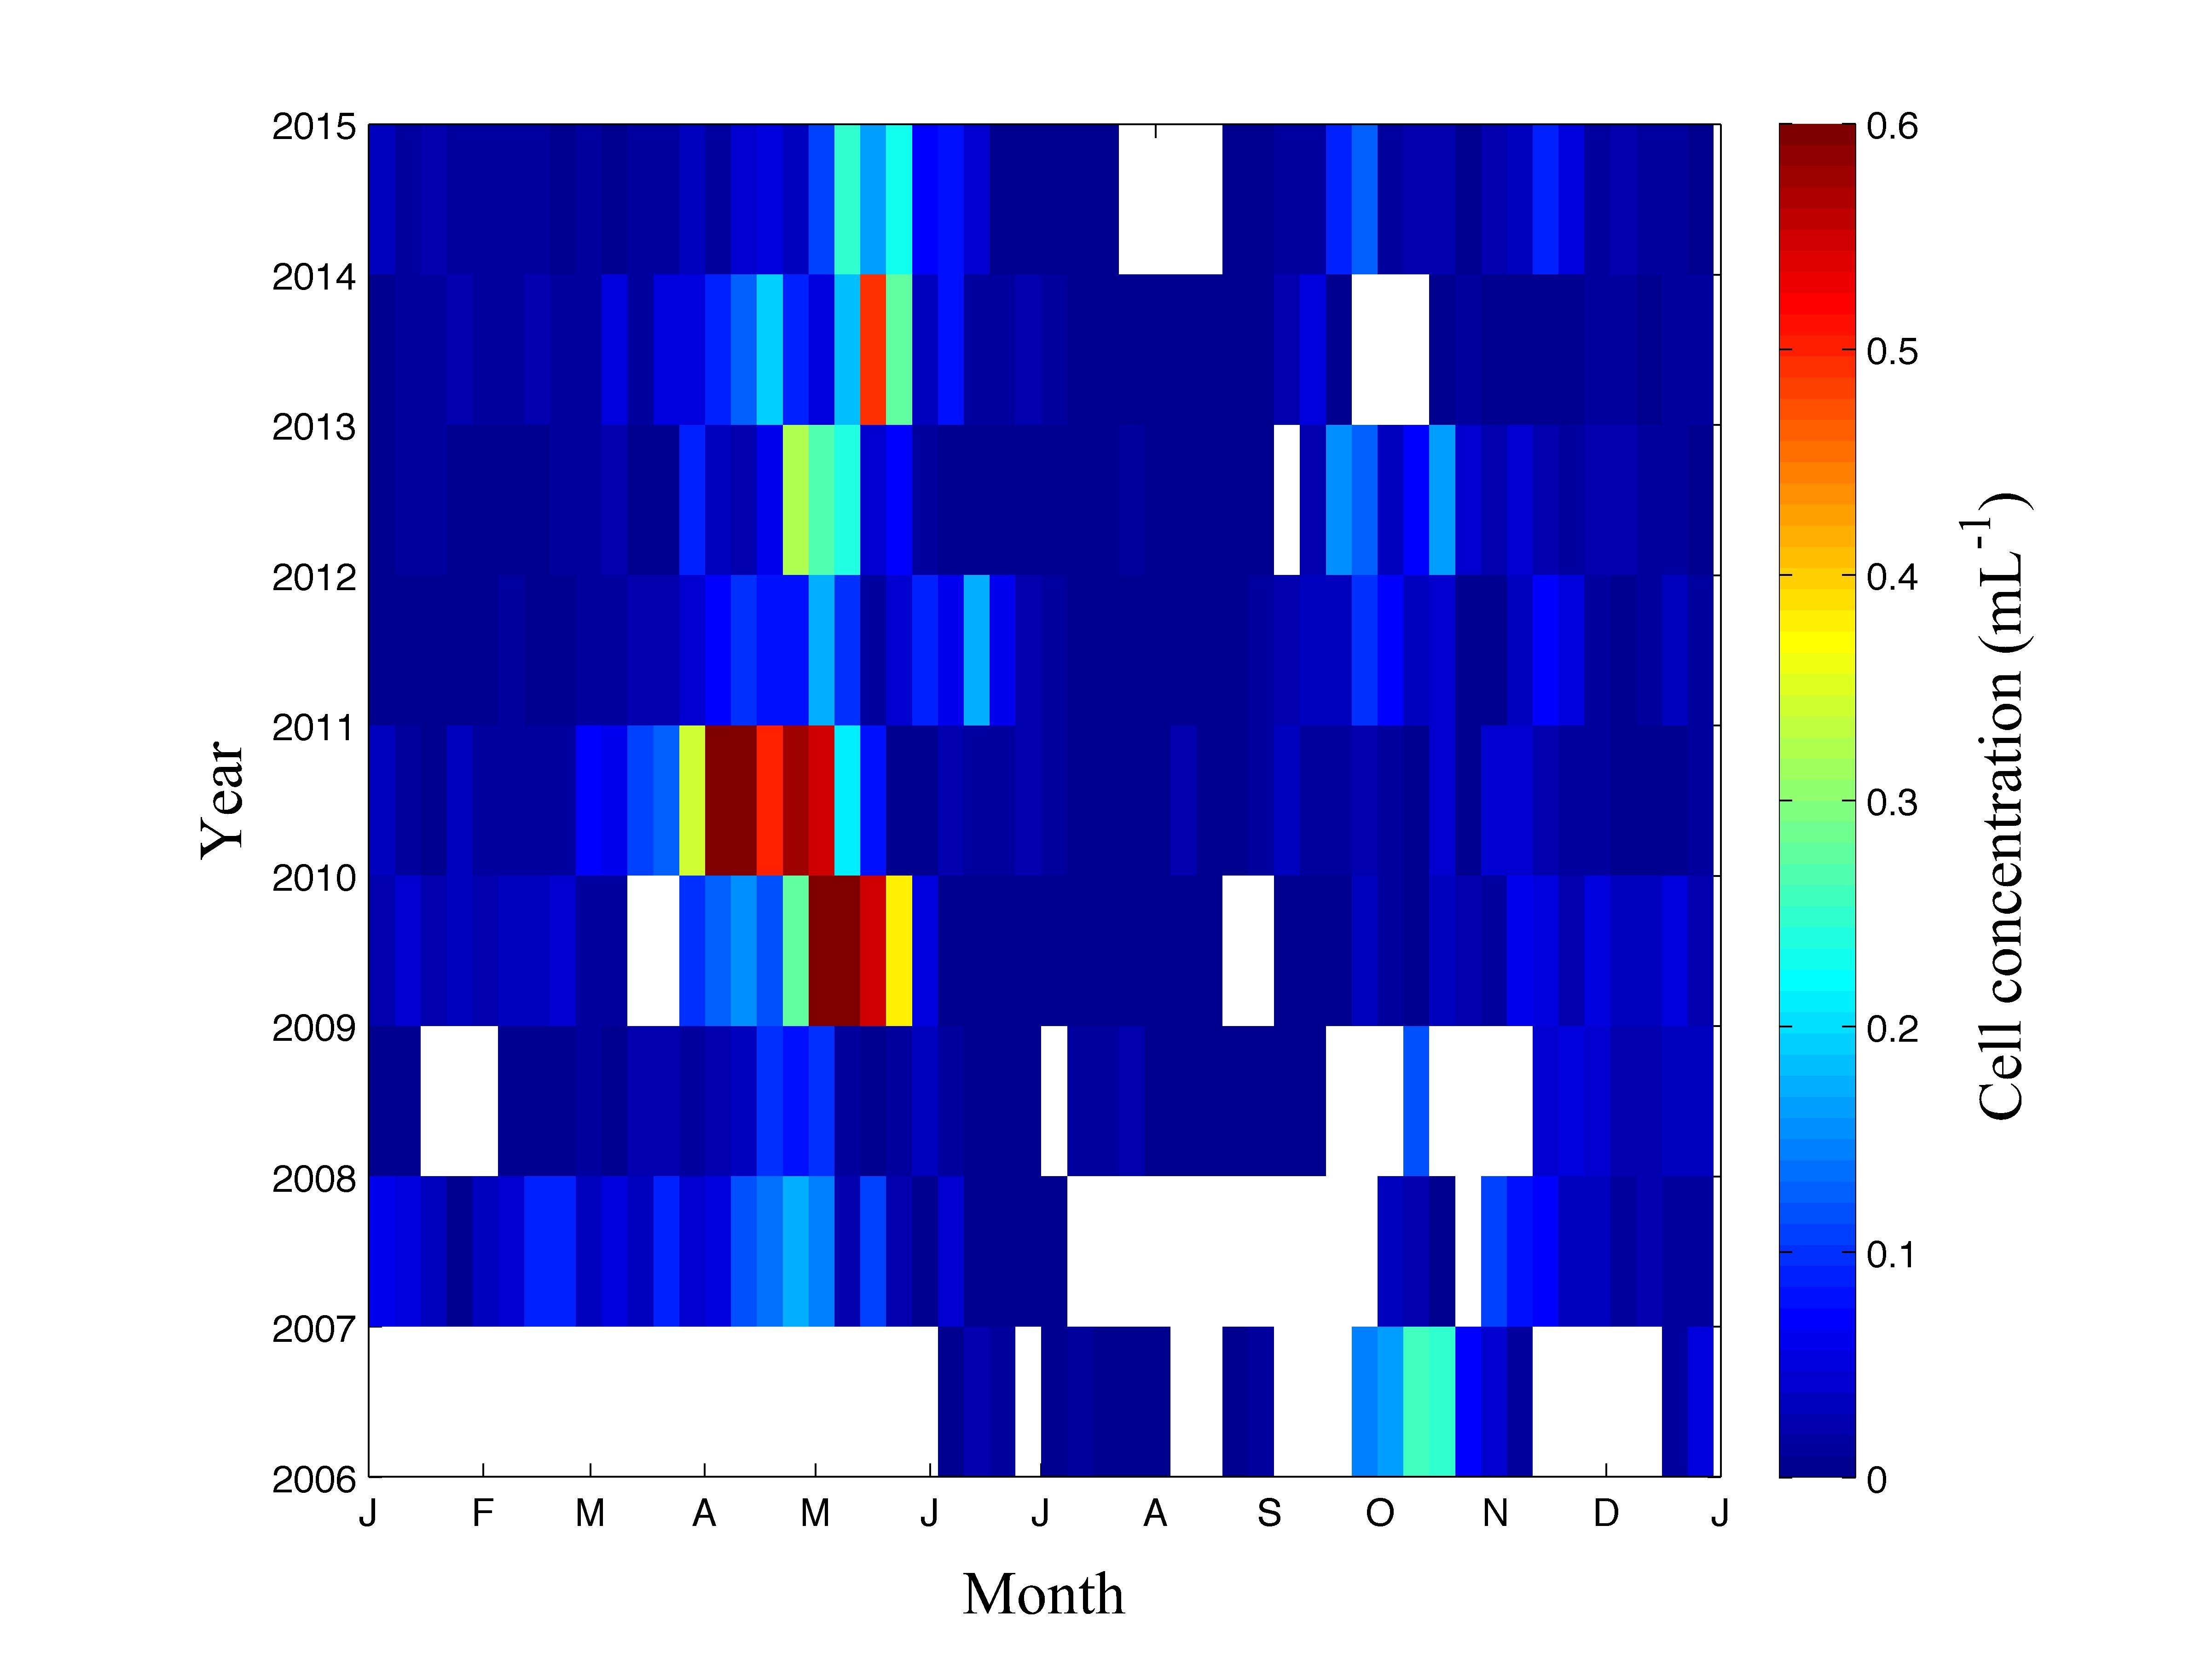
\includegraphics[scale=0.1]{laboea_seasonality_flat}
\caption [\textit{Laboea strobila} yearly seasonality] {Multi-year records of weekly-binned \textit{Laboea strobila} abundance at MVCO determined by IFCB sampling combined with automated image analysis and classification. White bars indicate times when no data is available}
\label{arm:fig2}
\end{figure}

